% file: modeledsystems.tex

\chapter{Modeled systems}
\label{ch:modeledsystems}
The goal of this thesis is to study fracture of methane hydrates. In order to do that, I need to know the mechanical properties of the model I study. Since studies of mechanical properties of methane hydrates modeled with TIP4P/ICE+UAM are scarce, I start this chapter by working out even the basic properties of the model, such as Poissons ratio and Youngs modulus. In order to be sure that the methods I use to estimate the mechanical properties work, I first check them with known values for a Lennard-Jones crystal. 

\section{Shear viscosity and diffusivity of the water model}
I have not been successful in finding values for the shear viscosity and diffusivity of bulk liquid water modeled with TIP4P/ICE. To measure these properties, I run a simulation like the one I ran to calculate verify the same properties for the TIP4P/2005 potential. Figure \ref{fig:viscosity_green_kubo_tip4p_ice} shows the Green-Kubo relation for the viscosity using 5 independent pressure components from 4 indepentent simulations with different simulation box sizes. Based on these data, I estimate the shear viscosity of TIP4P/ICE to $\eta_{GK} = \text{\SI{1.63\pm 0.05}{\milli\pascal\second}}$. 

\begin{figure}
\centering
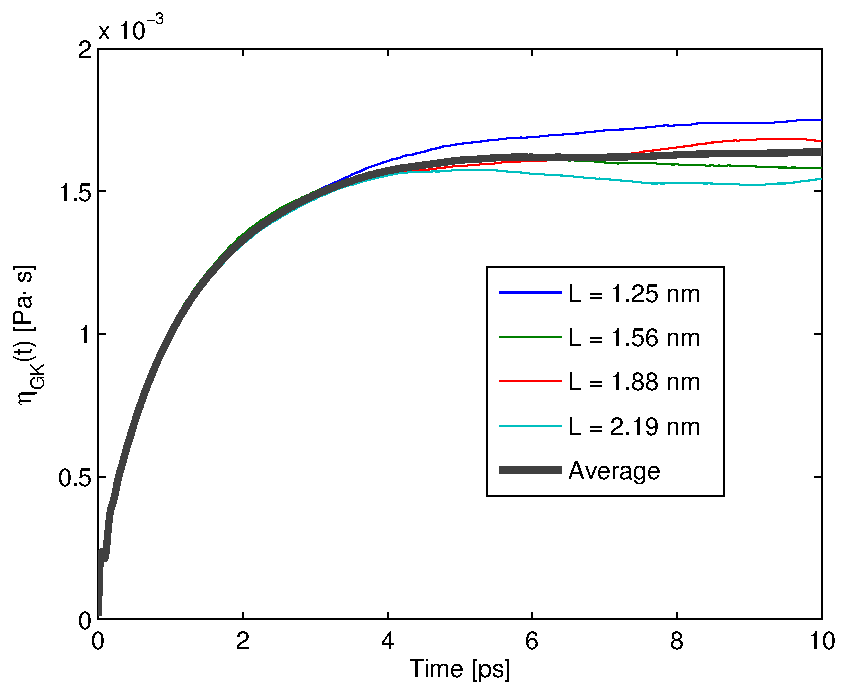
\includegraphics[width=10cm]{../figures/thesis/viscosity_green_kubo_tip4p_ice.pdf}
\caption{Shear viscosity for TIP4P/ICE at \SI{300}{\kelvin} and $\rho = \text{\SI{0.98}{\gram\per\cubic\cm}}$. Each thin line shows the average of the 5 independent pressure component. The thich line is the average of 4 independent simulations. The viscosity is estimated to $\eta_{GK} = \text{\SI{1.63\pm0.05}{\milli\pascal\second}}$}
\label{fig:viscosity_green_kubo_tip4p_ice}
\end{figure}

\begin{figure}
\centering
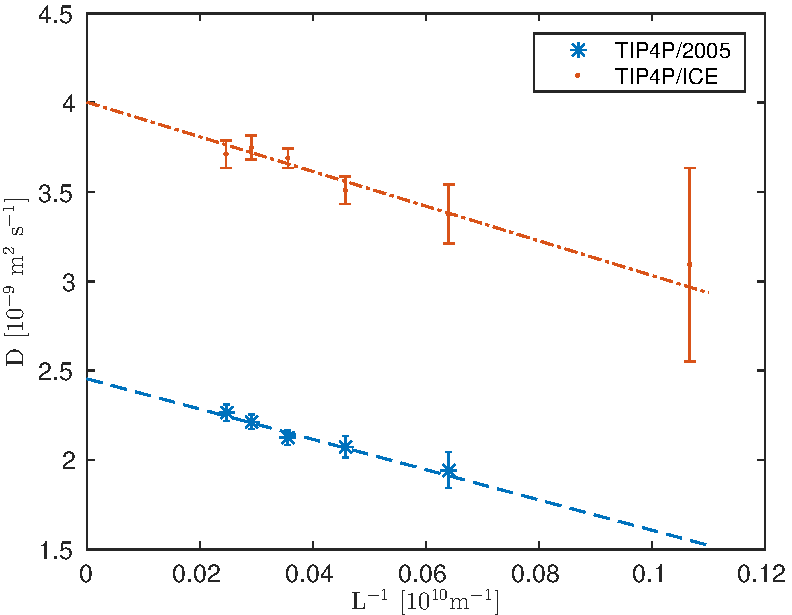
\includegraphics[width=10cm]{../figures/thesis/diffusivity_comparison_tip4p_ice_2005.pdf}
\caption{Linear regression of self diffusion coefficients as a function of inverse simulation box length. Results for TIP4P/2005 (blue) were already reported in the verification section. The self-diffusion coefficient for TIP4P/ICE is estimated to $D_0 = \SI{4.0 \pm 0.1 d-9}{\meter\squared\per\second}$}
\label{fig:diffusivity_comparison_tip4p_ice_2005}
\end{figure}

\section{Measuring elastic properties with a constant strain rate}
A naive approach, which i will use for crude estimates, is to subject a system to a constant strain rate by expanding the simulation box in one of the coordinate directions, and rescale all atom positions accordingly. An anisotropic thermo-barostat should be applied along the other axes, to keep the environment pressure and temperature constant. Since the barostat scales the simulation box, strains along the two axes perpendicular to the applied strain can be measured as the contraction of the simulation box in these directions:

\begin{equation}
\varepsilon_i = \frac{L_i-L_{0, i}}{L_{0, i}}
\end{equation}

If the sample is isotropic, I only have to simulate strain application in one of the coordinate directions to estimate both Young's modulus and Poissons ratio for a given system. To account for the possibility that the model I use do not exhibit isotropic behavior, I will check strains in both of the coordinate axes that are perpendicular to the axis of applied strain when calculating Poissons ratio. The scalar value of $\nu$ is the slope of the strain-strain curve, and for $E$ of the stress-strain curve, both in their linear regions. I will calculate these slopes using linear regression with least squares on the curves.
In the following, I will apply the method described above to a Lennard-Jones crystal and to the TIP4P/ICE+UAM methane hydrate model.

\subsection{Lennard-Jones crystal}
The FCC-lattice with a Lennard-Jones potential has been extensively investigated due to its simplicity. Therefore it provides robust benchmarking capabilities. I want to check that my protocols for dynamic (but quasistatic) determination of elastic properties and fracture strength reproduces known parameters for a Lennard-Jones solid. Reference values are for Young's modulus, $E=61.1 \epsilon/\sigma^3 = \text{\SI{2.40}{\giga\pascal}}$ (for the parameters I use for Methane), and for Poissons ratio, $\nu=0.347$. Values are taken from a molecular dynamics study by Quesnel et al. \cite{Quesnel1993}.

Figures \ref{fig:stress_strain_11_11_11_and_22_22_22_y_z_poisson_lennard_jones} and \ref{fig:strain_strain_11_11_11_and_22_22_22_y_z_poisson_lennard_jones} show data for a strain test of two systems of Lennard-Jones particles subjected to a strain rate of \SI{2d-8}{\per\femto\second} over \SI{0.8}{\nano\second} resulting in a maximum strain of \SI{0.8}{\percent}. The external pressure was set to \SI{50}{\mega\pascal}, and the temperature was \SI{5}{\kelvin}. Along with the data are estimates of Poissons ratio and Young's modulus, taken as the best linear regression with least squares. 


\begin{figure}
\centering
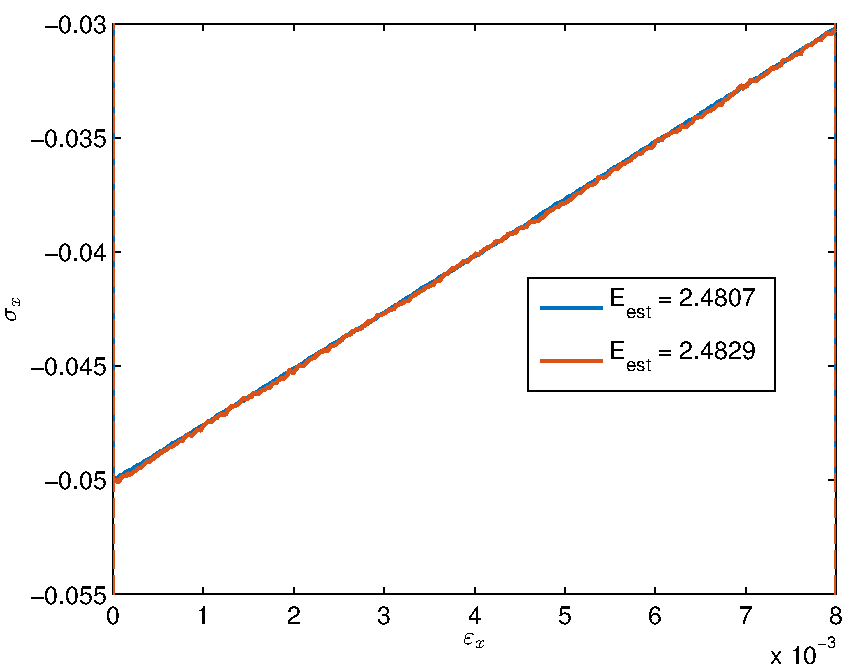
\includegraphics[width=10cm]{../figures/thesis/stress_strain_11_11_11_and_22_22_22_y_z_poisson_lennard_jones.pdf}
\caption{Stress-strain relations for Lennard-Jones systems of $11^3$ (red) and $22^3$ (blue) FCC unit cells. The sample was subjected to a constant strain rate of \SI{2d-8}{\per\femto\second}. $E$ is estimated using linear regression with least squares on all data points.}
\label{fig:stress_strain_11_11_11_and_22_22_22_y_z_poisson_lennard_jones}
% Path to simulation: /media/henriasv/Data/molecular-data/master_methane_hydrates/stress_strain/20150113_lennard_jones_strain
\end{figure}

\begin{figure}
\centering
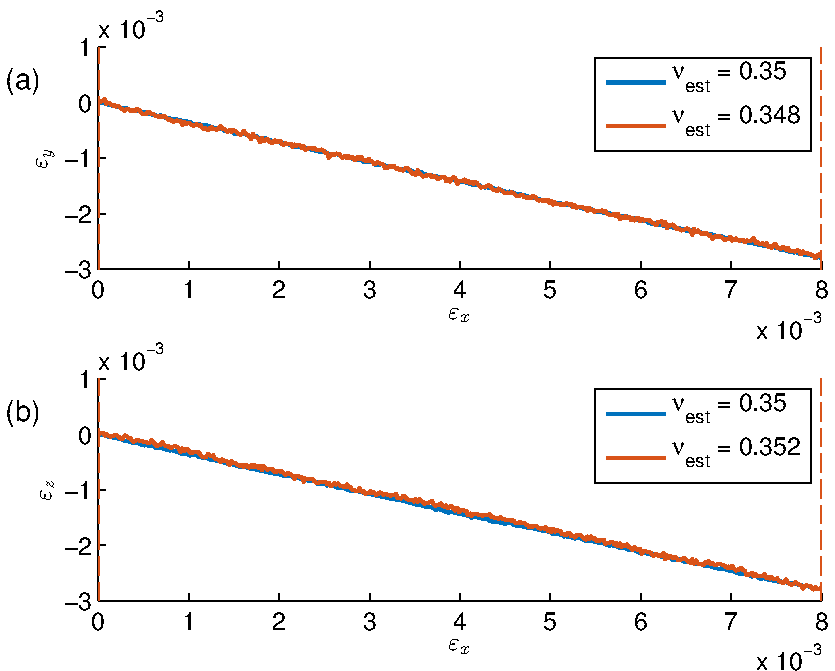
\includegraphics[width=10cm]{../figures/thesis/strain_strain_11_11_11_and_22_22_22_y_z_poisson_lennard_jones.pdf}
\caption{Strain-strain relations for for the same simulations as in Figure \ref{fig:stress_strain_11_11_11_and_22_22_22_y_z_poisson_lennard_jones}. All data points were used to estimate $\nu$.}
\label{fig:strain_strain_11_11_11_and_22_22_22_y_z_poisson_lennard_jones}
% Path to simulation: /media/henriasv/Data/molecular-data/master_methane_hydrates/stress_strain/20150113_lennard_jones_strain
\end{figure}

\subsection{S1 methane hydrate with TIP4P/ICE+UAM}
To my knowledge, there are no published estimates of Youngs modulus and Poissons ratio for the TIP4P/ICE+UAM model of methane hydrates. Therefore, I seek to make crude estimates of these quantities in dynamic simulations. I apply a constant strain rate by continously rescaling particle positions in one direction during MD-simulations. The other directions are kept under a constant pressure with anisotropic barostatting.
Figure \ref{fig:stress_strain_11_11_11_tip4p_ice_uam} shows the stress strain relationships and corresponding estimates of Youngs modulus for a system of 11x11x11 S1 unit cells subjected to strain rates of \SI{5d-7}{\per\femto\second} and \SI{2d-7}{\per\femto\second}. By extrapolating the results to quasistatic strain, Youngs modulus is estimated to \SI{7.1}{\giga\pascal}. 
Figure \ref{fig:strain_strain_11_11_11_y_z_poisson_tip4p_ice_uam} shows the relationship between applied strain along the x-axis and the measured strain along the other axes. It is not outrageous to assume S1 methane hydrate to be isotropic. Under this assumption, and by extrapolation to quasisatic strain, I estimate the poisson ratio for this model of S1 methane hydrate to be $\nu = 0.41$. 

\begin{figure}
\centering
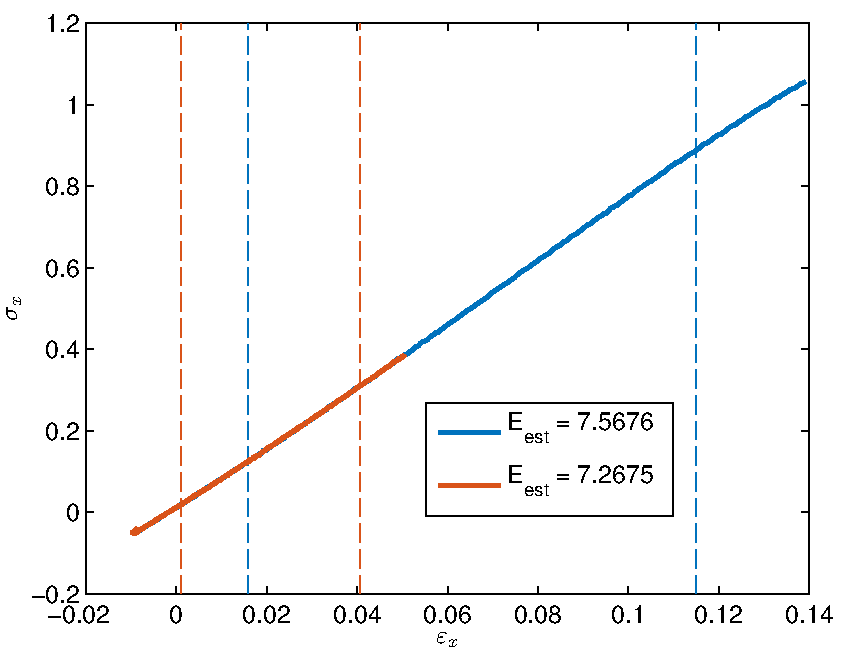
\includegraphics[width=10cm]{../figures/thesis/stress_strain_11_11_11_tip4p_ice_uam.pdf}
\caption{Stess-strain relations for a system of 11x11x11 S1 unit cells. Dashed lines indicate the region that was used to estimate Youngs modulus. Strain rates of \SI{5d-7}{\per\femto\second} (blue) and \SI{2d-7}{\per\femto\second} (red) along the x-axis. Upon close visual inspection, a slight rising slope can be seen for small strains and a rising slope for large strains, but overall the stress-strain relation is suprisingly linear, especially given the large strain-range.}
\label{fig:stress_strain_11_11_11_tip4p_ice_uam}
% Path to simulation: /media/henriasv/Data/molecular-data/master_methane_hydrates/stress_strain/20150108_youngs_modulus

\end{figure}

\begin{figure}
\centering
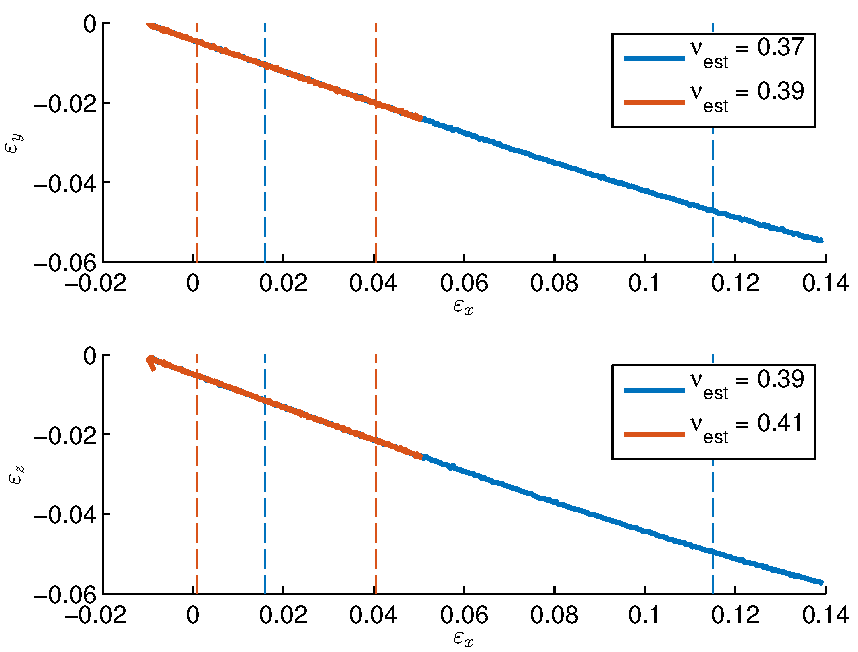
\includegraphics[width=10cm]{../figures/thesis/strain_strain_11_11_11_y_z_poisson_tip4p_ice_uam.pdf}
\caption{Strain-strain relations for the same system as in Figure \ref{fig:stress_strain_11_11_11_tip4p_ice_uam}. Measured strain along the y-axis (a) and z-axis (b) is plotted against the applied strain along the x-axis. Dashed lines indicate the region that was used to estimate Poissons ratio.}
\label{fig:strain_strain_11_11_11_y_z_poisson_tip4p_ice_uam}
% Path to simulation: /media/henriasv/Data/molecular-data/master_methane_hydrates/stress_strain/20150108_youngs_modulus

\end{figure}

\section{Early results on fracture and fracture toughness}



\subsection{Simulation protocol}
@VerifyThatThisIsADescriptionOfHantal2014
It is not at all obvious how to perform simulations to determine the fracture toughness. \citet{Hantal2014} performed NVT simulations and imposed a series of small deformations to their sample. After each deformation, they minimized the system, and then ran molecular dynamics for \SI{10}{\pico\second}. I have tried to use the same protocol, but find that for my system, the impact on the energy distribution among the degrees of freedom is too large when performing minimizations between the deformations. this results in a system farther out of equlilibrium that the deformed but not minimized system. Therefore, a possible protocol:

\begin{enumerate}
\item Equilibrate the system NVT (Molecular dynamics)
\item Perform small deformation
\item Reequilibrate the system NVT (Molecular dynamics)
\item If the strain i low: Return to 2. If the strain is high: continue.
\item Molecular dynamics run to wait for failure
\item If failure does not occur, or crack length stabilizes: Return to 2. 
\end{enumerate}

However there are problems here: The waiting time when waiting for failure must be carefully chosen, and if it turns out that critical and sub-critical failure are hard to distinguish, or even impossible to define, then waiting times can be arbitrarly long. 

From the latter discussion, I propose to exploit the possible time problem, and investigate the dependence on strain and temperature on the crack velocity and the waiting time before fracture occurs. The latter is possibly computationally expensive to get sufficient statistic to make any confident statements. 

A simpler protocol -- and I believe this to be a good way to study this particular system -- is to subject the sample to a constant strain rate, then wait for a crack to propagate. This is simple to do, and is also close to experimental conditions. The downside is that the loading is varying during fracture, disturbing measurements of properties like crack velocity at constant loading. It is, however, reasonable to believe that at low strain rates, these effects will be small, if not negligible. This can also be solved by setting the strain rate to zero at some predefined strain level, which is estimated from experience, and can be systematically varied. 


\subsection{Proof-of-concept simulations}
Before performing serious simulations, I do preliminary simulations to find out whether the protocol proposed in the latter section can produce interesting results. I do simulations on a relatively small and quasi two-dimensional system -- the system is only one unit cell thick -- to keep computational costs down. The total computational cost for tuning in on parameters and getting rid of bugs and blunders has been about $10^4$ cpu hours.

Figure \ref{fig:proof_of_concept_crack} shows the potential energy and strain for four simulations where S1 methane hydrates of 24x24x1 unit cells were gradually subjected to a strain of between 0.045 and 0.1 (see figure caption for simulation details). Then, the system was left on its own. In three of the systems, a crack spanned the yz-plane after the simulation was finished. The two others had seen no visible crack growth.

\begin{framed}
\paragraph{Visual experience of the crack propagation}
First, the system slightly contracts (NPT allows volume change). The system comes to rest, and some methane molecules diffuse out of near-wall cages to the hole that was carved out during initiation. After \SI{100}{\pico\second} straining starts. The system expands along the x-axis at a constant rate during \SI{50}{\pico\second},which corresponds to a very high strain rate if though of in macroscopic terms. More methane fills the crack, as its volume increases when the crack gets wider -- but the crack length remains the same during expansion. The system has now reached is the desired strain. Methane molecules bounce back and fourth inside the crack, and the crack edges seem jittery. Suddenly, a hydrogen bond near a crack tip breaks -- flucuations from methane molecules and lattice vibrations have made the system unstable. When the first bond breaks, the next bond along the crack axis can't hold it. Bonds near the other crack edge breaks. Then bonds break one after the other on both edges of the crack -- the crack propagates. In a matter of tens of picoseconds, both crack edges reach the periodic boundary. During crack propagation, clathrate cages are ripped apart. Water molecules remain stuck to the wall, while methane is released, and fills the void between the two pieces of methane hydrate (well, actually, because of the periodic boundary, there is still only \emph{one} piece of methane hydrate). The crack is not traveling straight in one direction: It first starts traveling between columns of sI cells before it turns and continues to propagate in the middle of hydrate cells, ripping apart big cages. Just after the crack has propagated, the methane hydrate oscillates with a spatial amplitude of the same order as the void width. During the following hundreds of picoseconds, the oscillations damp out -- the system is approaching a new equilibrium.
\end{framed}

From the visuals, I move on to preliminary calculations of the surface energy and the critial energy release rate. The surface energy can be estimated as the change in potential energy from the equilibrated system before straining to the system of methane hydrate and free methane after crack propagation. The energy release rate can be estimated as the change in potential energy during crack propagation. If $\Delta U_c$ is the change in potential energy during crack propagation, and $\Delta U_s$ is the change in potential energy from befor straining to after crack propagation, then the formulas for $G_c$ and $\gamma_s$ read:

\begin{equation}
	\mathcal{G}_c \approx \frac{\Delta U}{L_yL_z}
\end{equation}

\begin{equation}
	\gamma_s \approx \frac{\Delta U}{2 L_y L_z}
\end{equation}

Where the $\frac{1}{2}$ factor is because the crack opens two surfaces. The thermalization for all four of the simulations are equal, with an average potential energy of $\SI{-2.8112}{\femto\joule}$ on the plateau (40--100 \si{\pico\second}). The average potential energy after crack propagation was $\SI{-2.7970}{\femto\joule}$, with almost no variation among the simulations. This yields an energy difference of \SI{1.42d-17}{\joule}. Using the simulation box side face area (measured values: $L_y = \SI{288.8}{\angstrom}$, $L_z = \SI{12.04}{\angstrom}$) as an estimate of the crack size, the estimated surface energy is $\gamma_s = \SI{0.204}{\joule\per\meter\squared}$. Since the energy level required to start a crack is not well defined from figure \ref{fig:proof_of_concept_crack}, the critical energy release rate estimate is coarser. Reading off a potential energy of around \SI{-2.765}{\femto\joule}, the estimated critical energy release rate is \SI{1.3}{\joule\per\meter\squared}. This corresponds to, using equation \ref{eq:energy_release_to_stress_intensity_isotropic} for the stress intensity in isotropic materials, a critical stress instensity factor of $K_{Ic} = 0.10 \text{ MPam}^{\frac{1}{2}}$ (Using $E=\SI{7.1}{\giga\pascal}$ and $\nu = 0.4$). Unfourtunately, we shall see that this method for finding the fracture toughness is wrong because of how the energy was measured. More about that later in the chapter. For reference, the fracture toughness of real freshwater ice is around $K_{Ic} = 0.10 \text{ MPam}^{\frac{1}{2}}$. 

\begin{figure}
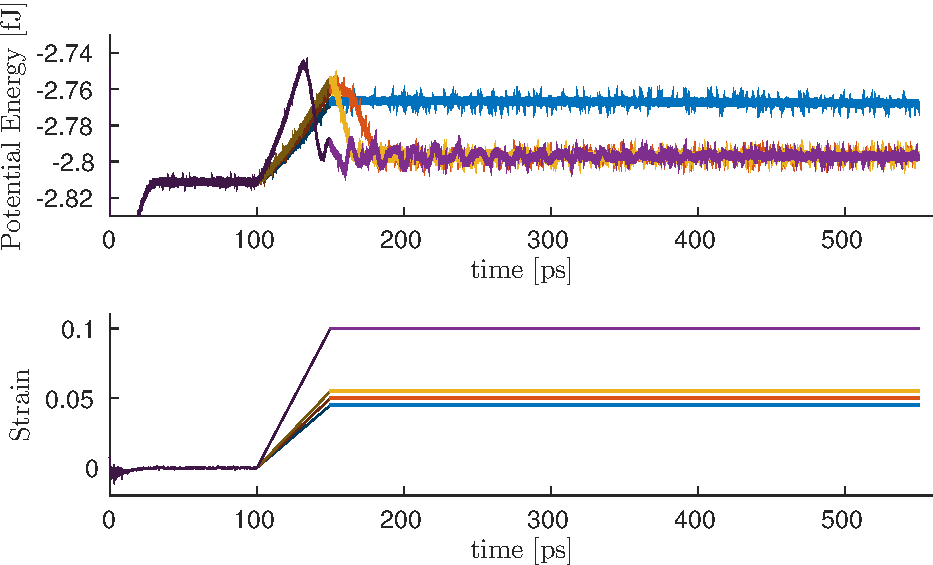
\includegraphics[width=\textwidth]{../figures/thesis/proof_of_concept_poteng_strain.pdf}
\caption{Potential energy (upper panel) and strain (lower panel) for a series of simulations where systems of 24x24x1 unit cells S1 hydrate are subjected to tensile strain. The systems were initiated with an elliptic crack of $6.0 \times 40.0 \si{\angstrom}$. The system was allowed to equilibrate NPT during \SI{100}{\pico\second}, which can be seen from the small fluctuations in strain in this timeframe. Then the simulations were NVT, but with imposed volume change due to the application of a constant strain rate, taking the system to a predesignated stress after \SI{50}{\pico\second}. Then, a regular NVT-simulation was run for \SI{400}{\pico\second} (bright colors). The thermostat and barostat damping times were \SI{1000}{\pico\second}. $T=\SI{260}{\kelvin}$. Falling potential energies correspond to crack opening (in these specific simulations). The slope of falling potential energy is systematically steeper for higher values of the strain before crack propagation. The systems that crack show oscillating potential energy after crack propagation, which is due to global oscillations of the system. The oscillations are damped out by a drag term in the thermostat. }
\label{fig:proof_of_concept_crack}
\end{figure}

\paragraph{Detailed crack analysis}
This is the point at which I developed my code to measure the crack area. Hopefully, that estimate will be better than the estimate solely based on the simulation box dimensions. The code also lets me follow the crack area in time, which makes it possible to measure the crack speed. I choose to define the crack speed as the change of crack area divided by the crack width, since the crack is well defined – it is $L_z$ of the simulation box. Keeping in mind that my cracks travel in two directions, the crack velocity for a crack initiated as a hole parallell to the z-axis is:

\begin{equation}
v_c = \frac{1}{2L_z}\frac{\dd A_c}{\dd t}
\end{equation}

@MeasureCrackInTimeForTheseSimulations

\paragraph{Summary of concept simulations} The results from this initial simulation indicate that methane hydrate under these conditions are very brittle on the tens-of-picoseconds scale, in the sense that they do not at all plastcally deform to withstand strain. They either deform elastically, or they fail. There is also indications that the time before fracture depends on the applied strain in a systematic way. A close look at the potential energy curve of the simulation in figure \ref{fig:proof_of_concept_crack} that did not end in rupture reveals that the potential energy is actually slowly decreasing. Whether this is a sign of a coming fracture, strengthening rearrangements of particles -- which could imply some ductility -- or something else, remains to be investigated. 

\subsection{Arising questions}
Several quiestion arise as a result of the proof-of-concept runs:
\begin{itemize}
\item Is the amount of methane that is freed during fracture propagation always the same?
\item Is there a relationship between the waiting time from straining ends till rupture starts and the slope of the potential energy curve?
\item Is the slowly decreasing potential energy of long waiting-time events important, and can it be related to the waiting time?
\item What is the fracture toughness for long (infinite) waiting times, and is it possible to measure? Will the system melt before it fractures?
\item Is the methane in the initial crack important for fracture initiation?
\end{itemize}

There are also several technical problems that can be addressed:
\begin{itemize}
\item What is the effect of the thermostat damping time on fracture properties?
\item Is the strain rate important? Does the time it takes to strain the system compete with the waiting time until fracture?
\end{itemize}

Each of these questions will require substantial efforts to be answered, and I will only have time to address a few of them. In the sections to come, I focus on @insertHere. I will essentially ignore the technical issues for now. If I find something interesting, the tecknical issues will of course be part of the verification -- but I find it unjustifiable to spend time and cpu core hours on these issues before I have found anything interesting that needs thorough verification.

\section{Energy considerations -- the thermodynamics of expanding the simulation box}
The result that $\mathcal{G}_c > 2\gamma_s$ to the extent that was seen from the preliminary results is peculiar -- and actually wrong. In the last section, I only considered the potential energy to estimate the fracture toughness, since fracture mechanics dictates that the fracture toughness should be the amount of potential energy released per projected crack surface area opened. But really, it is the Helmholtz free energy release rate that should be used for fracture toughness calculations -- potential energy in fracture mechanics is not necessarily the same as in molecular dynamics. A more thorough analysis solves the problem of methane hydrates seeming very brittle while having $\mathcal{G}_c > 2\gamma_s$, and the conclusion, which we shall see, is that we actually have $\mathcal{G}_c \approx 2\gamma_s$.

Let's consider expanding the simulation box along the x-axis. This corresponds to perform work on the system:

\begin{equation}
	W = \int_{t(L_x = L_x^0)}^{t(L_x^0 + \Delta x)} \int_{yz} \sigma_{xx} (t, y, z) \ \dd z \dd y \dd x
\end{equation}

If the system is in equilibrium, then:
\begin{equation}
\int_{yz} \sigma_{xx} (t, y, z) \ \dd z \dd y = L_yL_z\Sigma_{xx}(t)	
\end{equation}
Where $\Sigma_{xx}$ is an element of $\uuline \Sigma$, which is the mean stress tensor for particles in the system. The work on the system can then be written:

\begin{equation}
	W = L_y L_z \int_{t(L_x = L_x^0)}^{t(L_x^0 + \Delta x)} \Sigma_{xx}(t) \ \dd x
	\label{eq:work_expansion}
\end{equation}
This expression can easily be extracted from a molecular dynamics simulation.
In the canonical ensemble (NVT), the change of internal energy will be:
\begin{equation}
	\Delta U = W + T\Delta S
\end{equation}
When expanding the system, the entropy per temperature will increase, as more microstates are available. This has to be compensated by adding heat. In molecular dynamics, the thermostat effectively adds energy as entropy during simulation box expansion. Furtermore, this energy cannot increase the kinetic energy, since N and T are kept fixed, so all the added heat must be absorbed as \emph{potential} energy. This means that expanding the simulation box adds a lot of potential energy to the system, both directly through mechanical work, and indirectly through heat. Storage of the mechanical work is in line with the intuition -- particles are positioned higher in each others potentials. The heat absorption is more subtle: The system creates more available microstates when it expands homogeneously at a constant temperature. These microstates do only exist because of the strained state of the system, and will disappear if the strain disappears, for example during fracture. The entropy energy is not available for mechanical work. This is why Helmholtz free energy should be considered:

\begin{equation}
	F = U - TS
\end{equation}

This is exactly the energy available for mechanical work. The reason for this tedious discussion of expanding a box is that Helmholtz free energy is not directly available from molecular dynamics simulations. The change in Helmholtz free energy must be explicitly done by integrating the stress tensor of the system. When analyzing fracture, it would be tempting to use the change in total energy or potential energy to estimate the fracture toughness. But this would be wrong -- the fracture toughness should be caclculated using the available mechanical energy. The energy release rate is the amount of Helmholtz free enegry needed to create projected crack surface area, not the change in potential or total energy of the system during fracture. This distinction is not easy to see when reading fracture mechanics, as fracture mechanics usually deal with elastic bodies with no temperature, but it is crucial when studying fracture in molecular dynamics.

When the crack propagates, the stress in the methane hydrate is released, and the system consists of a piece of methane hydrate and some free gas in between. We don't know the entropy of this system, but it seems reasonable from the strain energy compared to the potential energy that the change in entropy from before straining to after fracture is small compared to the strain energy -- unless the system was strained significantly more than necessary.


\citet{Hantal2014} proposes to calculate the critical energy release rate with the following formula (This method was used for illite with ClayFF and ReaxFF):
\begin{equation}
	\mathcal{G}_c = V \frac{\int_0^{E_{\text{final}}}\uuline{\Sigma}(E) : \dd \uuline{E}}{\int_0^{E_{\text{final}}} \dd A_{crack}}
	\label{eq:hantal_critical_energy_release_rate}
\end{equation}


This is in principle sufficient to determine the critical energy release rate for any mode of loading, provided that the conditions for using Equation \ref{eq:hantal_critical_energy_release_rate} to estimate the critical energy release rate are met. 
For expansion of the simulation box along the x-axis, the strain integral (nominator) is equivalent to \ref{eq:work_expansion}. The area integral (denominator) is just the crack area in time, which can be estimated using the crack tracer described in @ref. 

%%%%%%%%%%%%%%%%%%%%%%%%%%%%%%%%%%%%%%%%%%%%%%%%%%%%%
\section{Large simulations of fracture}
%%%%%%%%%%%%%%%%%%%%%%%%%%%%%%%%%%%%%%%%%%%%%%%%%%%%%

\subsection{Complete analysis of a single simulation}
\label{sec:complete_analysis_single_simulation}
In this subsection, I use the analysis tools that were presented in the tools section to analyze \emph{one} simulation. This simulation will be referred to as the \emph{full-analysis simulation}. The analyzes here will be representative of how data is obtained when showing up in later results where data from several simulations are used together to say something more general.

\begin{figure}
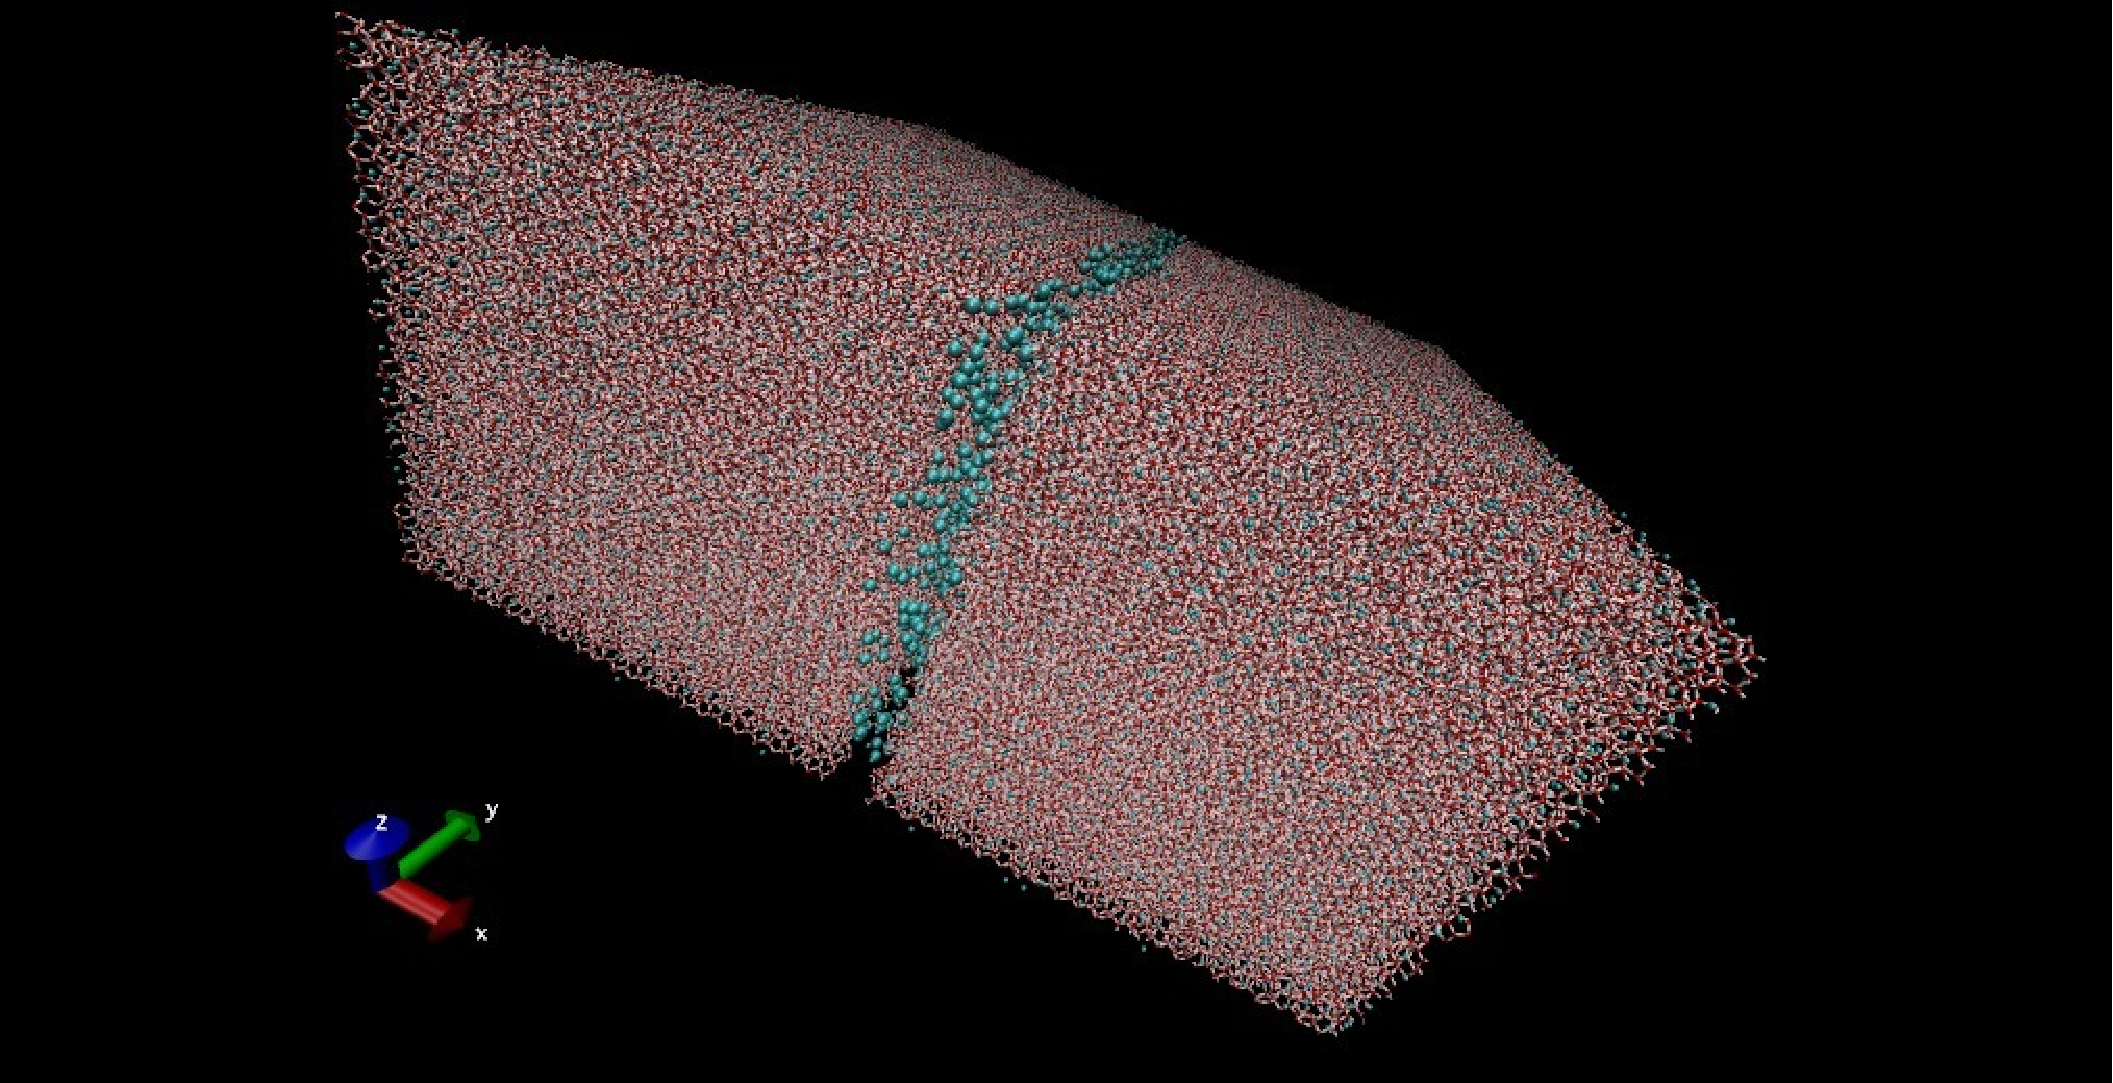
\includegraphics[width=\textwidth]{../pictures/system_1048.pdf}
\caption{Perspective image of a representative state after fracture in a $24\times 24 \times 12$ sI unit cell simulation. The biggest green spehres are methane molecules that are considered free to move (not enclathrated). Smaller green spheres (barely visible) are enclathrated methane molecules. Water molecules are drawn as hydrogen bonds.}
\label{fig:system_1048}
\end{figure}

\begin{framed} 
\textbf{Simulation details:} A system consisting of $24 \times 24\times 12$ S1 unit cells is prepared. First, an elliptical hole in the xy-plane spanning the whole z-direction is carved out as described in section \ref{subsec:reg_eprism}. The system is then allowed to equilibrate with an anisotropic NPT thermo-barostat for \SI{100}{\pico\second}, with ambient barostat pressure (\SI{101325}{\pascal}). The system is then integrated NVT, but subjected to a constant strain rate taking it to a strain level of $\epsilon_{xx} = 0.048$ after \SI{50}{\pico\second}. Then straining is stopped, and the system is left NVT for \SI{350}{\pico\second}. The damping time of the thermostat and barostat during the whole simulations is $t_{damp} = \SI{1}{\ps}$. Additionally, a drag coefficient of $1.0$ (as described in the LAMMPS documentation) is added, as this is recommended to damp oscillations in solids. The thermostat temperature is set to \SI{260}{\kelvin}.
\end{framed}

For illustrative purposes, figure \ref{fig:system_1048} shows what the system looks like in perspective. The other pictures are rendered with an orthographic projection, so the system will look two-dimensional. 

Figure \ref{fig:crack_evolution} shows the evolution of the crack in time, to give an idea of what the system looks like during fracture. 

Figure \ref{fig:energy_1048} shows the potential energy, the kinetic energy and the strain energy for the whole simulation. It shows that a strain of 0.048 is only a bit more than what is needed if the the criterion for a crack to propagate is $\mathcal{G}_c = 2\gamma_s$. That means the system shows brittle behavior in this particular simulation. The kinetic energy slightly increases, which means the temperature increases during fracture. This is beacuse the release of heat is faster than what can be absorbed by the thermostat. The temperature is not indicated in the figure, but the temperature change is only by a few Kelvin. 

Figure \ref{fig:stressfield_avg_wait_for_crack} shows all components of the stress tensor of the system in space in the period where the system is fully strained, but before propagation starts. It is averaged over the z-direction in space and over \SI{20}{\pico\second} in time to get statitsics for a nice picture. The stress field is visually compatible with the analytical solution close to the crack tip for a homogeneous isotropic linear elastic solid. The shear components normal to the xy-plane are small, but not negligible That means the plane strain condition is only partially met. Particularly, the amplitude of $\tau_{xz}$ is about $1/5$ of that of $\tau_{xy}$. 


Figure \ref{fig:stressfield_snap_propagation_180} is similar to figure \ref{fig:stressfield_avg_wait_for_crack}, but it now shows the stress field during crack propagation Since tracking the crack requires higher time resolution, the stresses are only averaged over \SI{0.3}{\pico\second}. As expected, the region of high stresses moves along with the crack tip.

Figure \ref{fig:stressfield_timelapse} shows the stress $\sigma_{xx}$ at several points in time before, during and after crack propagation. Here also, the stresses are only averaged over \SI{0.3}{\pico\second}. The top crack is leading the bottom crack with $\sim \SI{10}{\angstrom}$, which is probably coincidental

Figure \ref{fig:crack_area_evolution_1048} shows the measured crack area in time, and its time derivative which estimates the crack tip speed. The maximum crack tip speed is around \SI{1}{\kilo\meter\per\second}. A little bump can be seen in the crack tip speed during crack propagation. This is a feature that always show up in simulations of the same system but with a different strain. My guess is that it is caused by bulk elastic waves triggered by the crack. The crack tip speed is a measure that is likely to be influenced by the strain level before fracture. 

Figure \ref{fig:free_methane} shows the system after fracture with the free methane -- methane that was released as a consequence of the crack -- indicated as big spheres. This figure is explained later, but the data is from this full-analysis simulation.

\begin{figure}
\begin{minipage}[b]{0.5\linewidth}
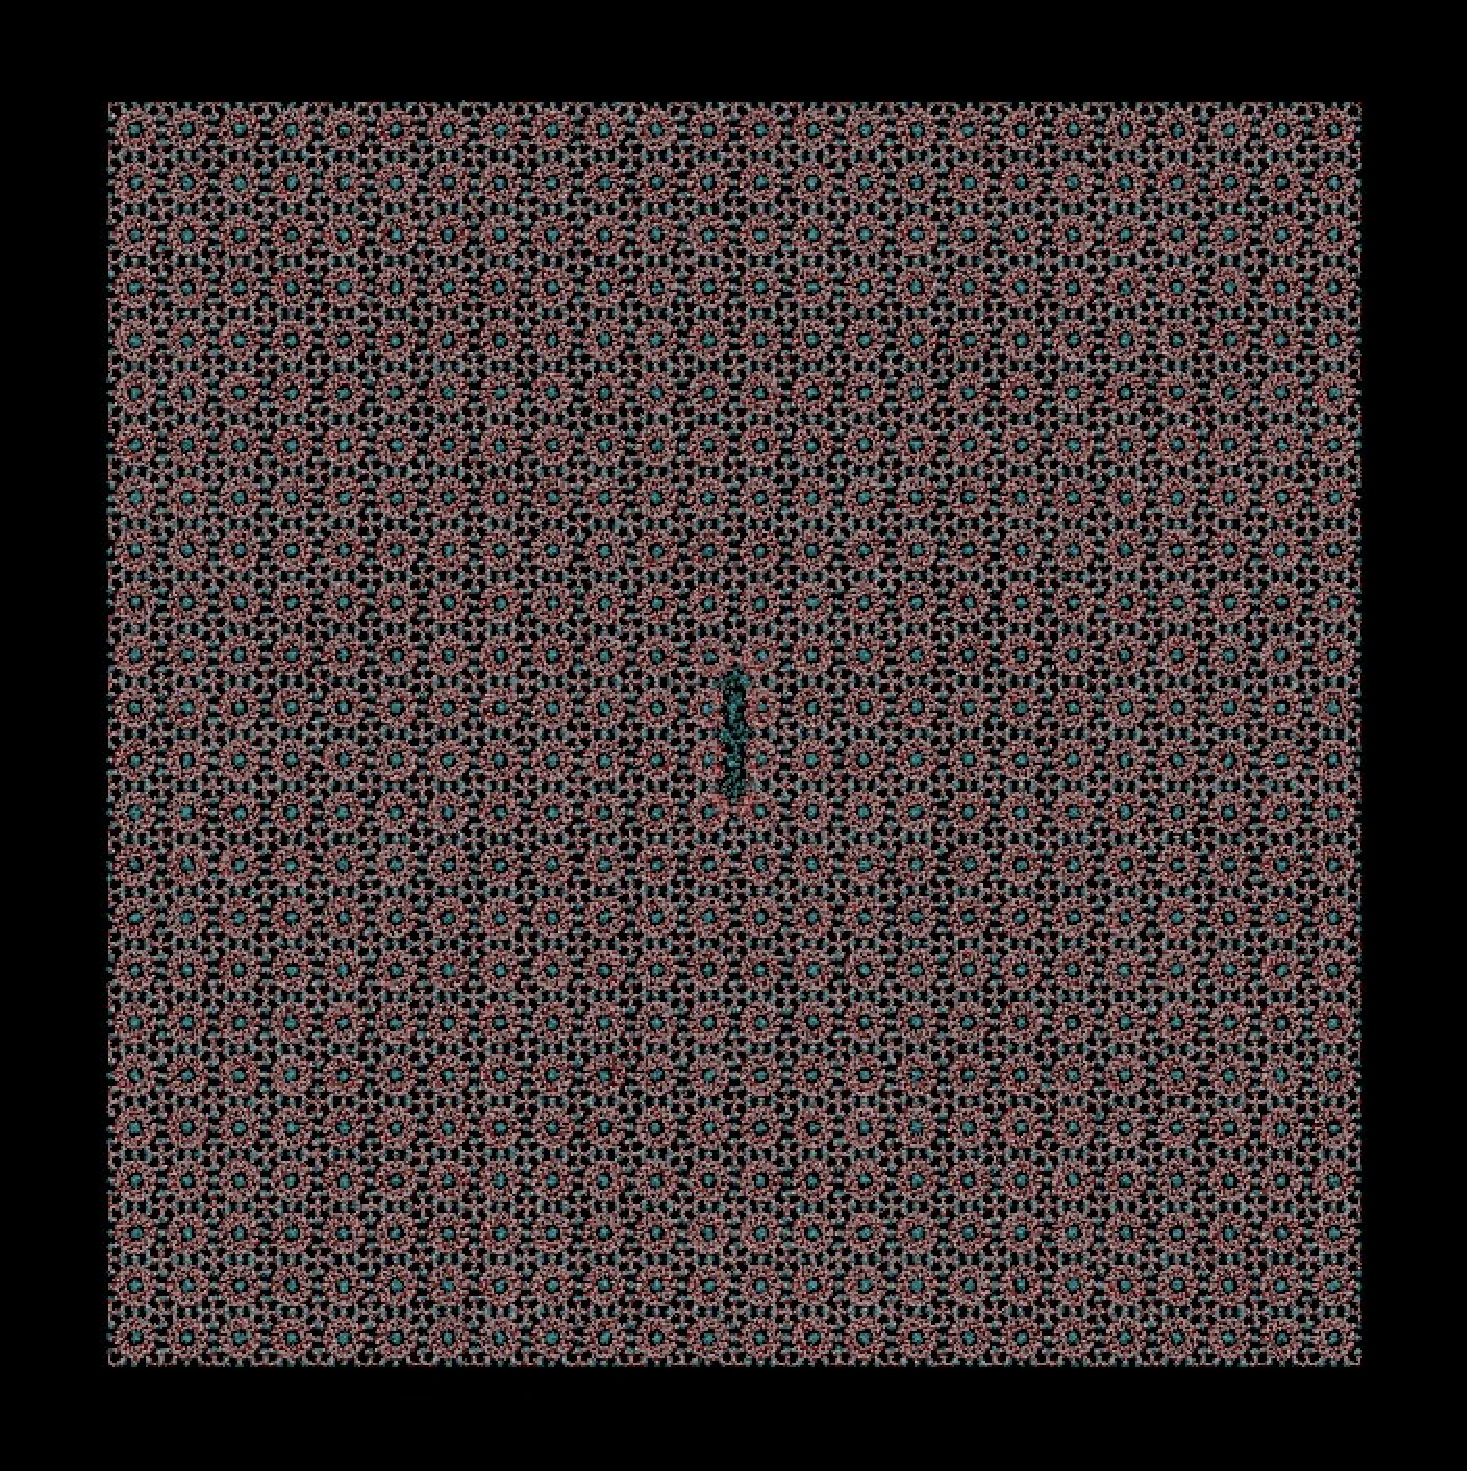
\includegraphics[width=\textwidth]{../snapshots/c_1.pdf}
\end{minipage}
\begin{minipage}[b]{0.5\linewidth}
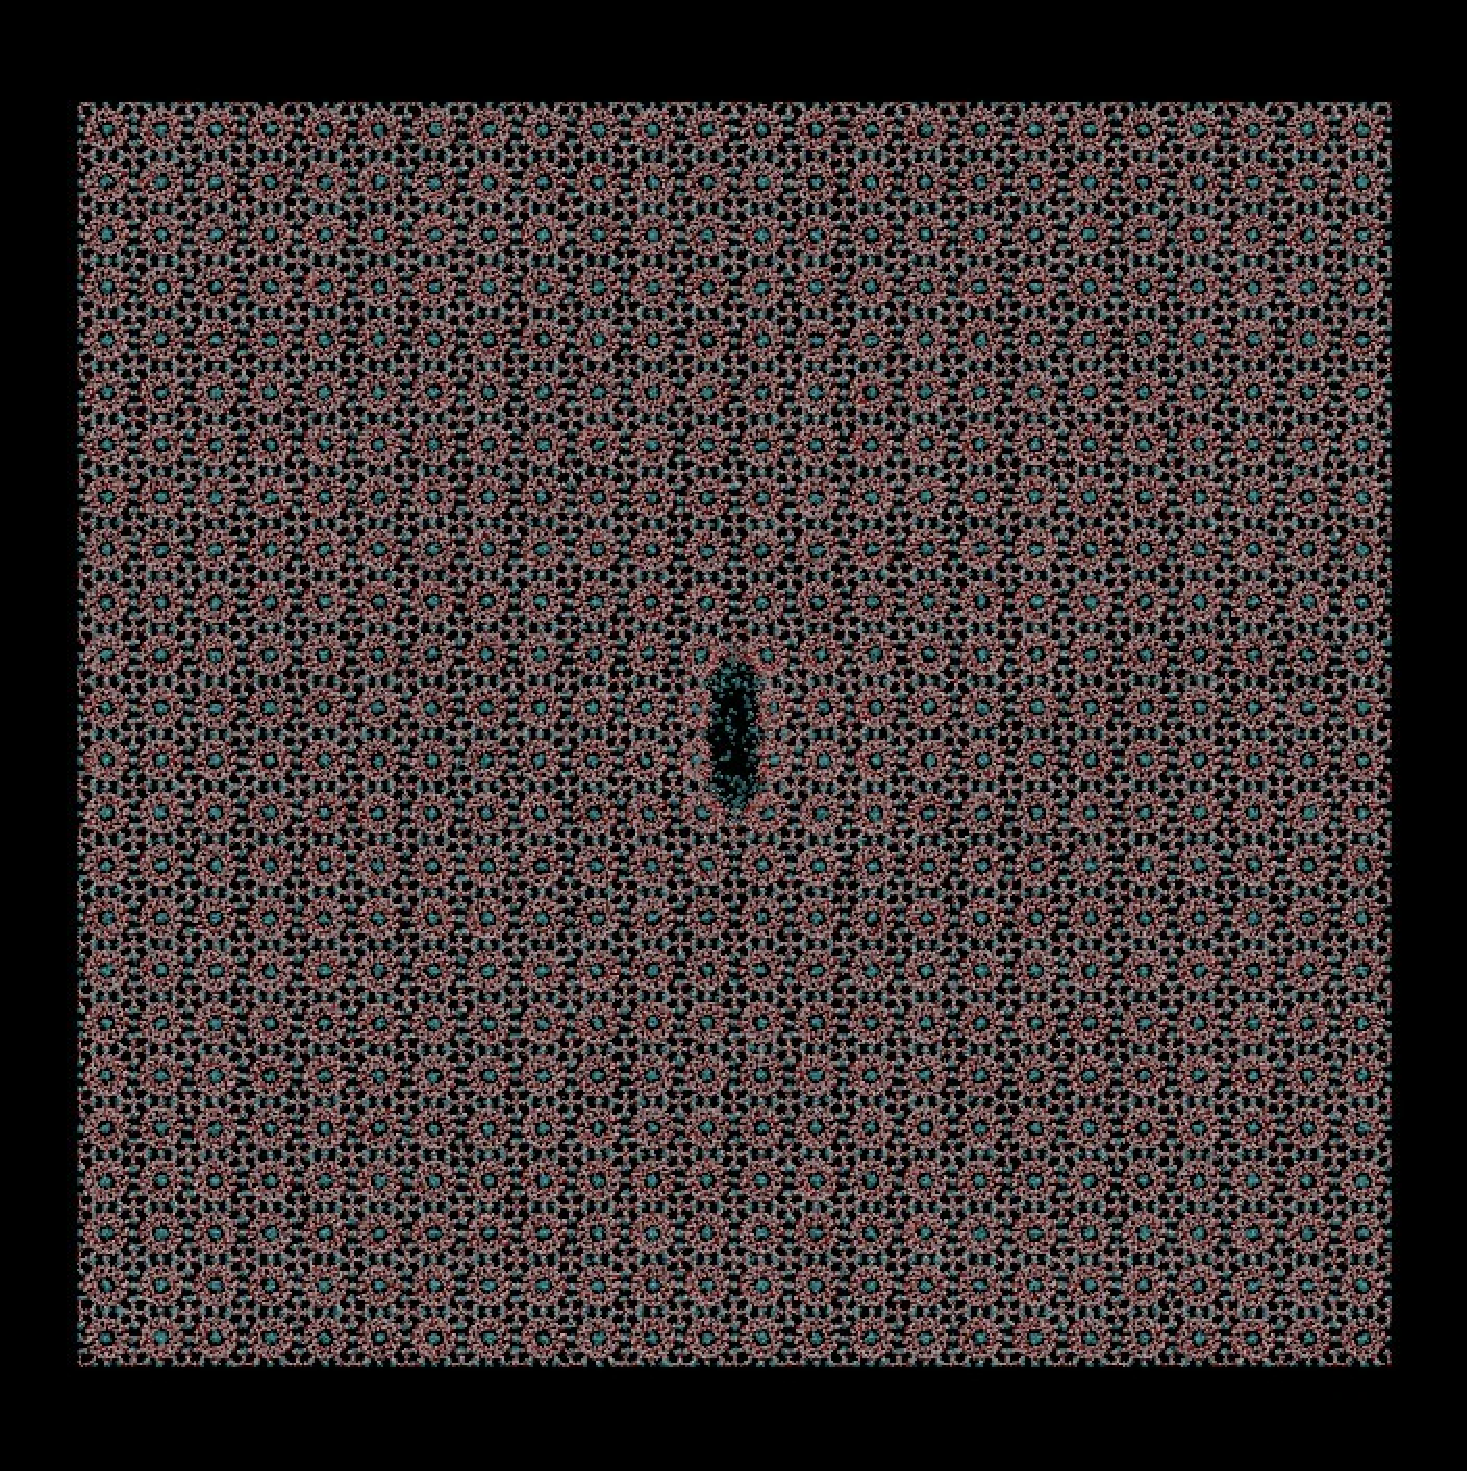
\includegraphics[width=\textwidth]{../snapshots/c_2.pdf}
\end{minipage}
\begin{minipage}[b]{0.5\linewidth}
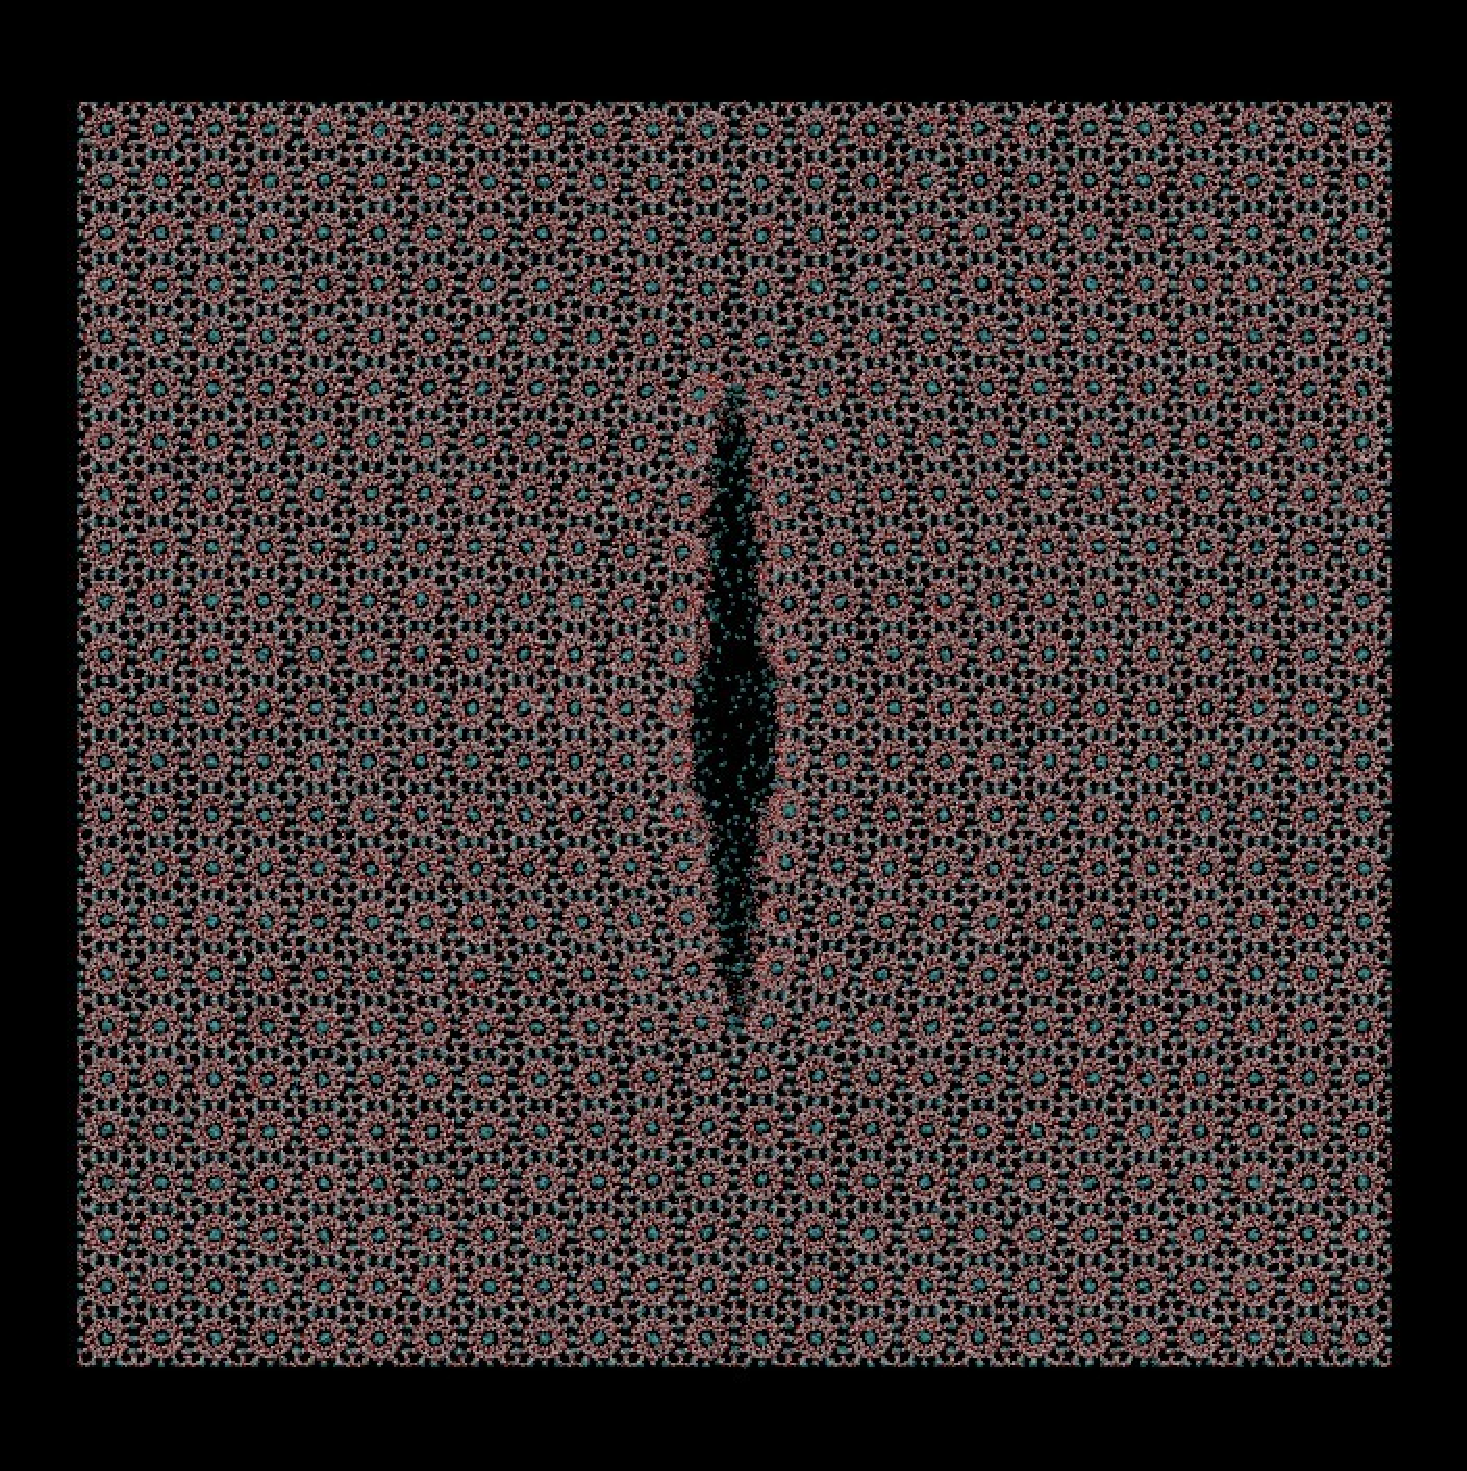
\includegraphics[width=\textwidth]{../snapshots/c_3.pdf}
\end{minipage}
\begin{minipage}[b]{0.5\linewidth}
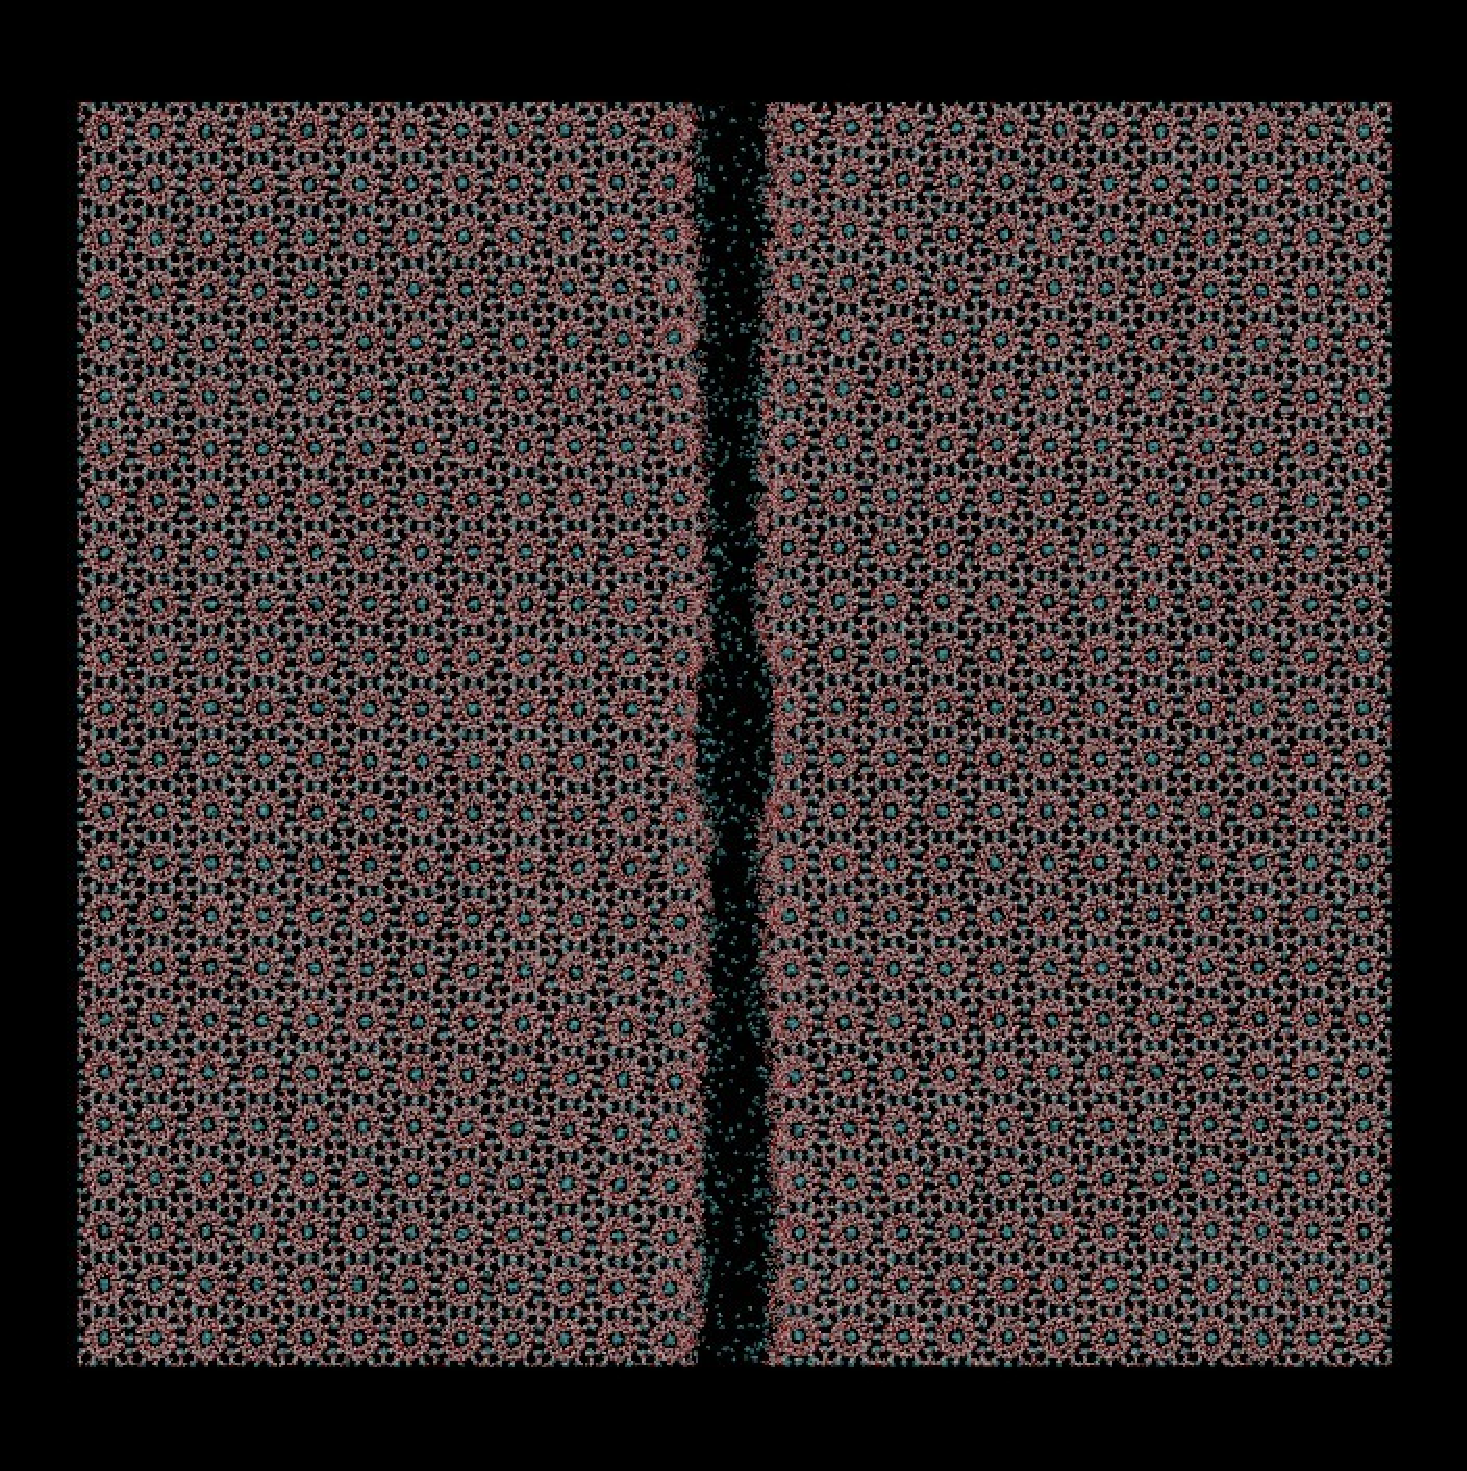
\includegraphics[width=\textwidth]{../snapshots/c_4.pdf}
\end{minipage}
\caption{(upper left) Equilibrated system, \SI{90}{\pico\second}. (upper right) Fully strained system ($\varepsilon_{xx} = 0.048$), \SI{150}{\pico\second}. (lower left) Crack started propagating, \SI{180}{\pico\second}. (lower right) Crack fully propagated after \SI{210}{\pico\second}. The crack is wider near the xz-plane periodic boundary at this point in time due to global oscillations following the crack propagation.}
\label{fig:crack_evolution}
\end{figure}


\begin{figure}
\centering
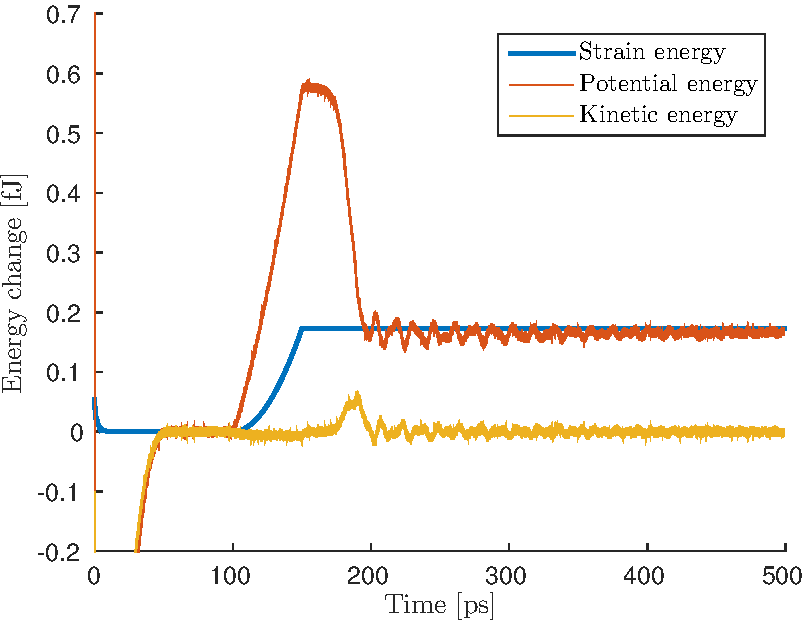
\includegraphics[width=10cm]{../figures/thesis/strain_pot_kin_eng_1048_24_24_12.pdf}
\caption{Strain energy, potential energy and kinetic energy for the whole 0.048 strain simulation. The values are rebased at $t=\SI{100}{\pico\second}$ where straining starts. The kinetic energy corresponds to the temperature, and we see that the temperature slightly drops while the strain increases, and increases during crack propagation. The strain energy imposed on the system is just slightly higher than the energy difference between the unstrained system and the fractured system.}
\label{fig:energy_1048}
\end{figure}

\begin{figure}
\centering
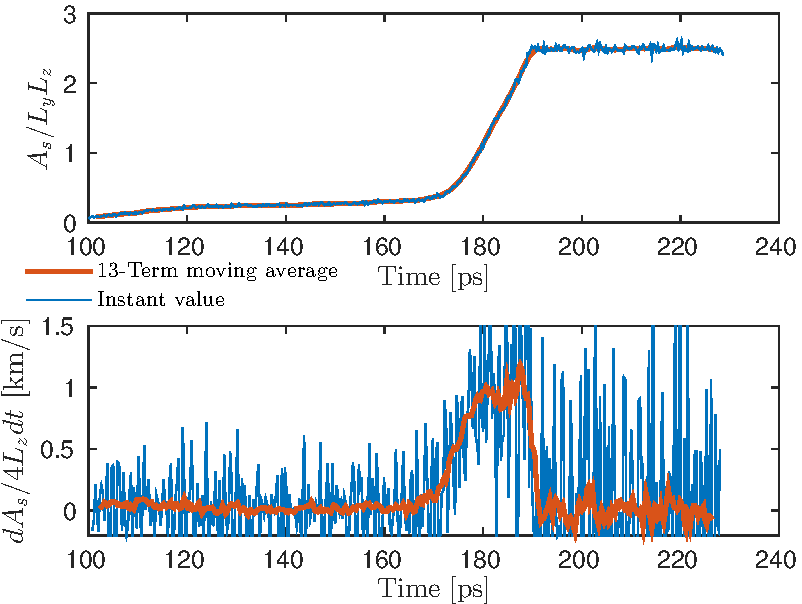
\includegraphics[width=10cm]{../figures/thesis/crack_area_evolution_1048.pdf}
\caption{Crack surface area evolution in time. The upper panel shows the measured area, and the lower panel is an estimate of the crack tip speed. The derivative for the lower panel is calculated using a standard 5-point stencil for the first derivative. The crack surface area was measured useing the Monte Carlo procedure described in section @ref with $N_s = 10^6$, $r_p = \SI{4.0}{\angstrom}$ and $\Delta l = \SI{1.0}{\angstrom}$. Note the little bump in the crack speed around \SI{180}{\pico\second}.}
\label{fig:crack_area_evolution_1048}
\end{figure}

\begin{figure}
\centering
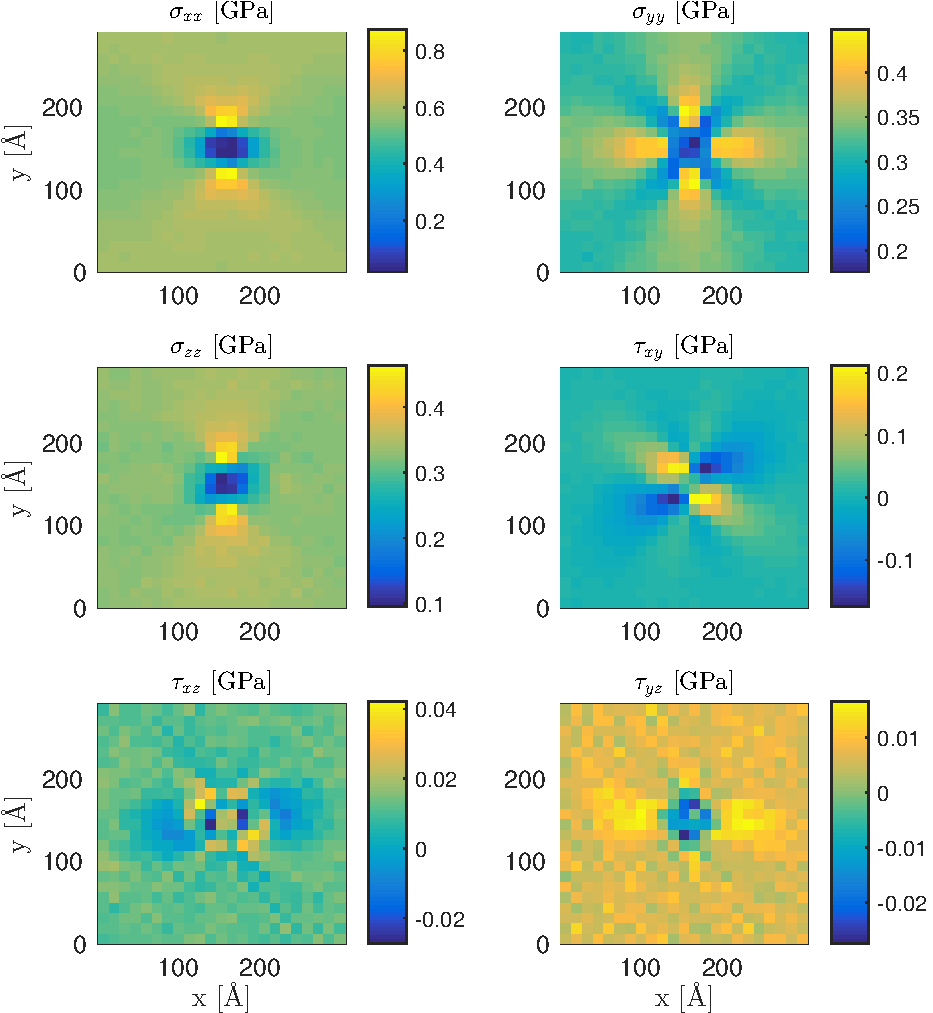
\includegraphics[width=\textwidth]{../figures/thesis/stressfield_avg_wait_for_crack.pdf}
\caption{Stess field averaged over \SI{20}{\pico\second} just after straining was stopped, and while waiting for a crack to start. The modeled system is $24\times 24\times 12$ S1 unit cells. The four uppermost panels show features qualitatively in line with the analytical solution of the stress field around the crack tip of elliptical hole in a linearly elastic and isotropic material. The shear stress components ouside the xy-plane are relatively small compared to the components in the xy-plane, which means the plane strain condition is satisfied fairly well. The stress fields near the crack tips are, at least qualitatively, similar to the analytical solution for isotropic materials given in figure \ref{fig:analytic_stress}. Note also the stress $\sigma_{zz}$ it looks like $\sigma_{xx}$ due to $L_z$ being fixed, disallowing poisson contraction.}
\label{fig:stressfield_avg_wait_for_crack}
\end{figure}


\begin{figure}
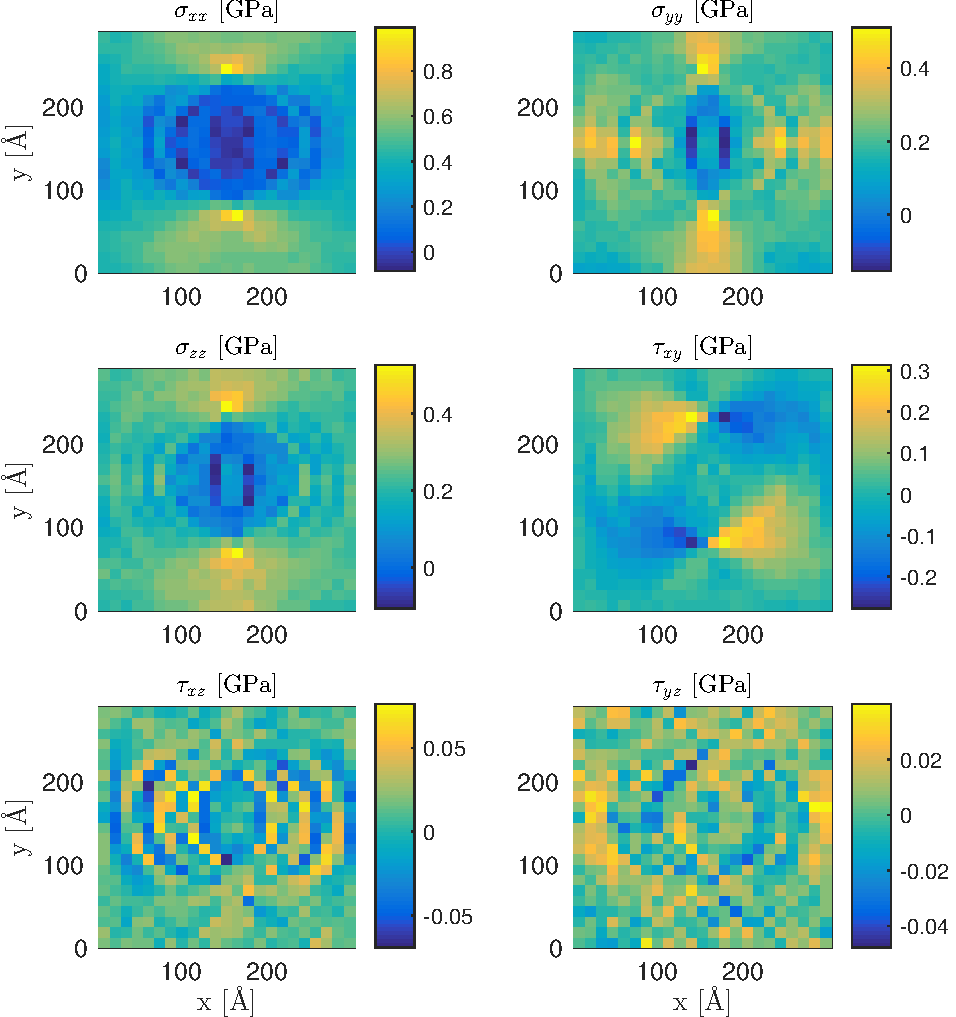
\includegraphics[width=\textwidth]{../figures/thesis/stressfield_snap_propagation_180.pdf}
\caption{Snapshot of stress field during crack propagation. Average over \SI{0.3}{\pico\second} before $t = \SI{180}{\pico\second}$.}
\label{fig:stressfield_snap_propagation_180}
\end{figure}


\begin{figure}
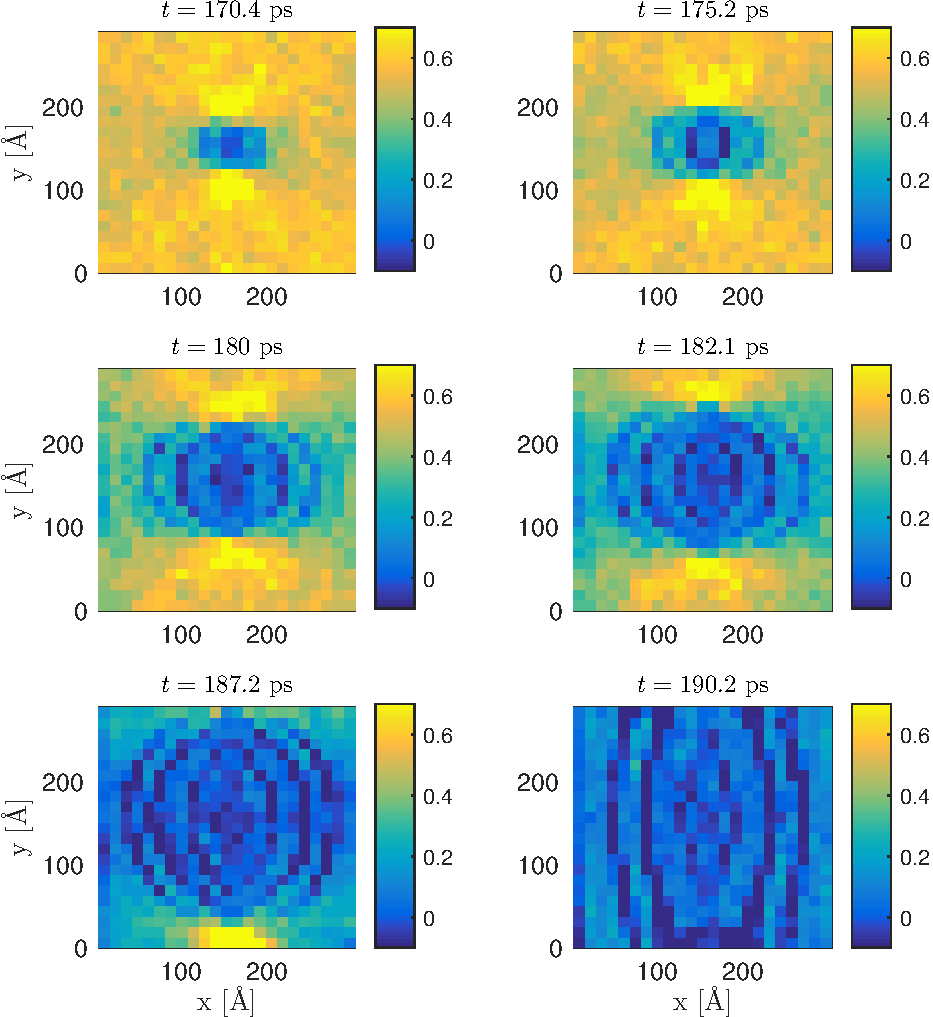
\includegraphics[width=\textwidth]{../figures/thesis/stressfield_timelapse.pdf}
\caption{Timelapse of the stress $\sigma_{xx}$ during crack propagation. There are clear signs of sound waves, and the shape of the waves indicate that the crack is traveling at a speen on the same order of magnitude as the shear wave speed. The color scale is kept equal among the simulations for easier comparison. For that reason, the stress near the crack tip is higher that what is available on the color scale. Notice that the two edges of the intial hole don't crack at the same time. The upper crack is leading the lower crack 
with $\sim \SI{10}{\angstrom}$. }
\label{fig:stressfield_timelapse}
\end{figure}




%%%%%%%%%%%%%%%%%%%%%%%%%%%%%%%%%%%%%%%%%%%%%%%%%%%%%%%%%%%%%%%%%%%%%%%%%%%%%%%%%%%%%
\section{A simple characterization of the fracture: The amount of free methane.}
%%%%%%%%%%%%%%%%%%%%%%%%%%%%%%%%%%%%%%%%%%%%%%%%%%%%%%%%%%%%%%%%%%%%%%%%%%%%%%%%%%%%%
I believe that the amount of free methane can be a valuable measure of how the crack surface looks because free methane no longer support a cage structure. Water molecules either stay on the crack surface, or are immidiately drawn towards the crack surface in a matter of picoseconds after a crack has passed. Methane, on the other hand, is free to move in the pore space created by the crack. A first order approach to crack surface characterization is therefore to count free methane in the pore space and use that to estimate the amount of hydrate that was dissociated during fracture. The simplest estimate is obtained by using the hydrate number $n_w$ (5.75 for fully occupied sI hydrate) to count the amount of water molecules that are no longer part of the stable hydrate structure. 


\subsection{Estimate by counting}
\label{sec:freemethane_counting}
A more straightforward approach, which is more computationally demanding, is to go through all methane positions, and check wheter they are part of the wall or the void, like what was done when tracking cracks. A particle is considered free if it was part of the void at any time during the simulation. The reason for the ``at any time during the simulation'' is that measuring frame by frame largely underestimates the number of free methanes. Methanes that are free arent necessarily far enough from the closest water molecule to be considered void, but they \emph{are} free to move. To check the that the free methanes are indeed free, the positions of the methanes that were defined as void can be visualized at a point in time after the crack has propagated. Since free methane is accumulated in the measurement, a slightly higher $r_p$ is needed than for crack tracing -- near the lower reasonable limit for $r_p$, some improbable (but they will occur in large simulations) wall configurations will result in wall methane beeing counted as free. Figure \ref{fig:free_methane} is a snapshot of the system with the free methanes highlighted. Some of the methane molecules that are considered free actually reside in small cages near the fracture surface, and it is not obvious wherer they should be considered free or not. I tend toward considering the free, since they have proven that they are in cages that are not sufficiently intact to keep the methane molecules over time. Most of the free methane molecules are clearly free, so this sould not be a big issue -- but it can be interesting to study for instance the rate at which methane is captured and released by the near-crack-surface cages.

\begin{figure}
\centering
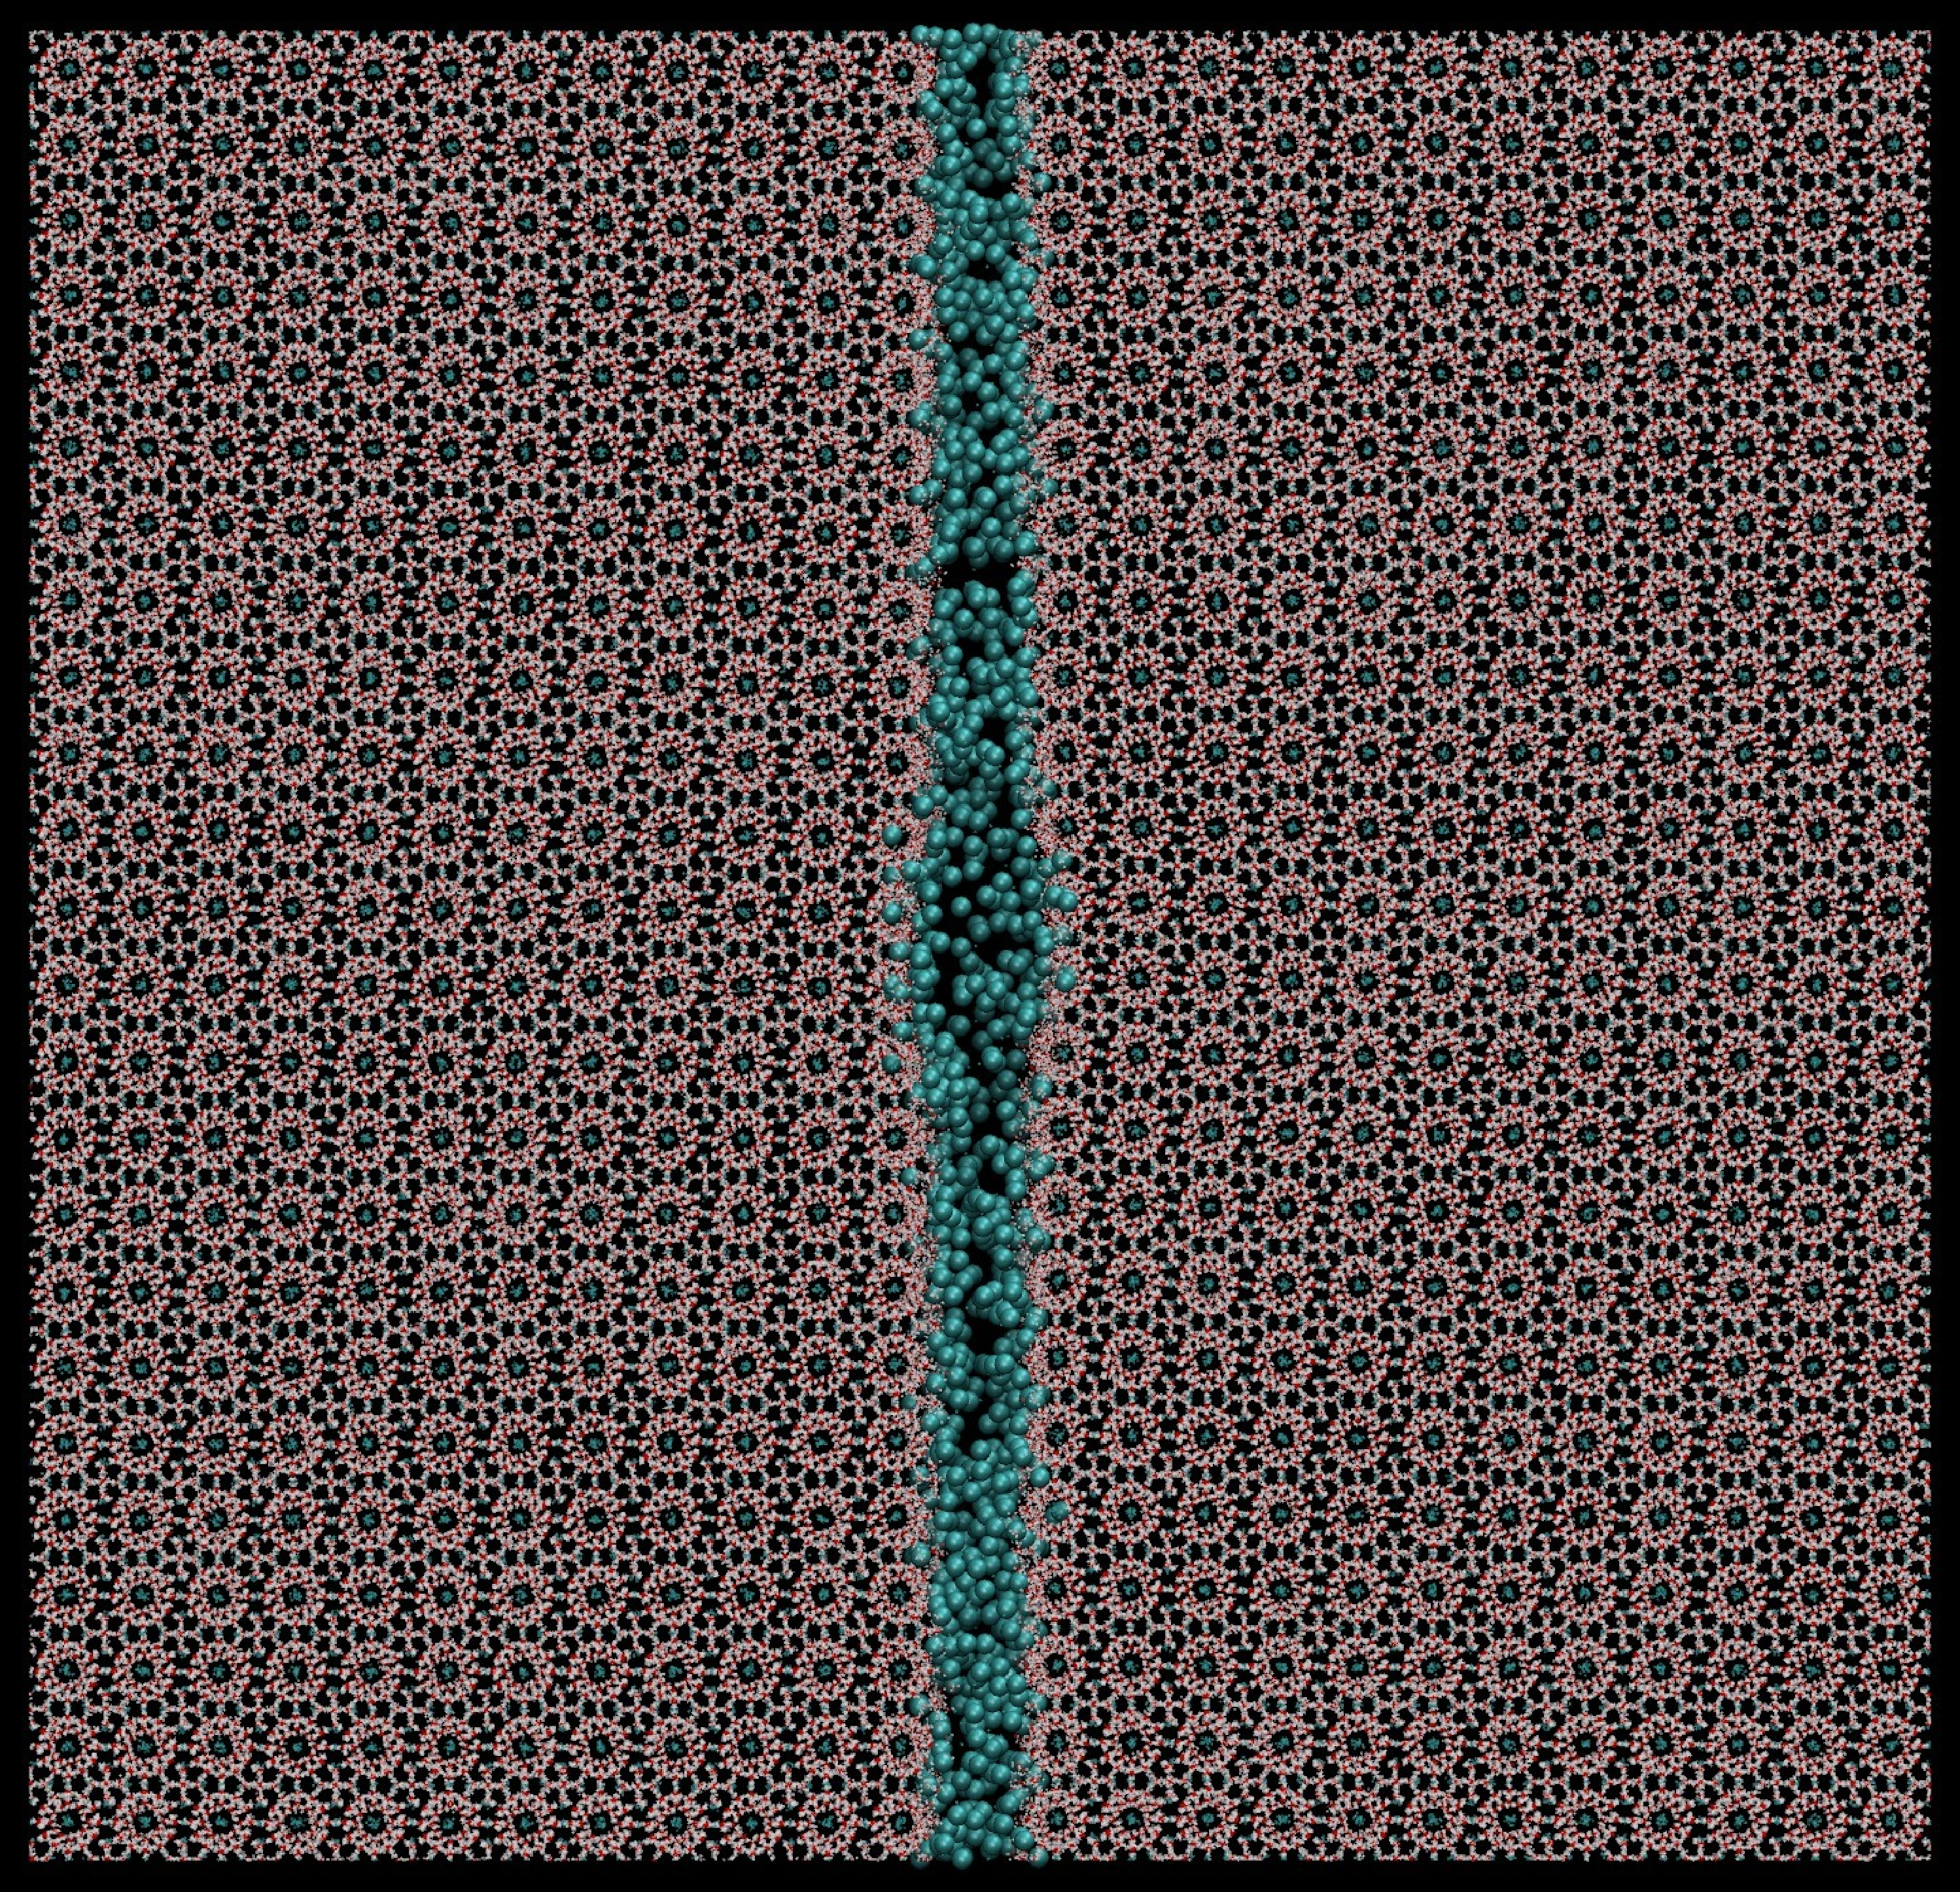
\includegraphics[width=\textwidth]{../pictures/free_methane.pdf}
\caption{Free methane -- particles that were more than $r_p = \SI{4.5}{\angstrom}$ away from any water molecule at some point -- are drawn as big green spheres. Other methane molecules are barely visible particles. Note that some ``free'' methane molecules actually occupy cages. Most of them are in the small nearest to the crack, but a few also occupy big cages, that are a bit farther from the crack surface. }
\label{fig:free_methane}
\end{figure}


\paragraph{Problems with this method}
\begin{itemize}
\item Some methanes jump in and out of clathrate cages. 
\item Instant number of free methanes is not available.
\end{itemize}

\subsection{Results on free methane}
Figure \ref{fig:free_methane_diff_l} shows the amount of free methane during simulation for two different thicknesses of the system. The number of free methanes is rescaled using the number of sI unit cells per cross section parallell to the crack. With full occupancy, the number of methanes per sI cell is 8, and if a whole plane of unit cells released their methanes, that would yield a number of 8 free methanes after rescaling. The number of free methanes shows no significant variance with the system thickness. This is a bit surprising, since the crack propagation has seemed more jittery for thinner systems, which could have led to mer methane being released. It might still be an effent, but in that case the effect must be small. 

\begin{figure}
\centering
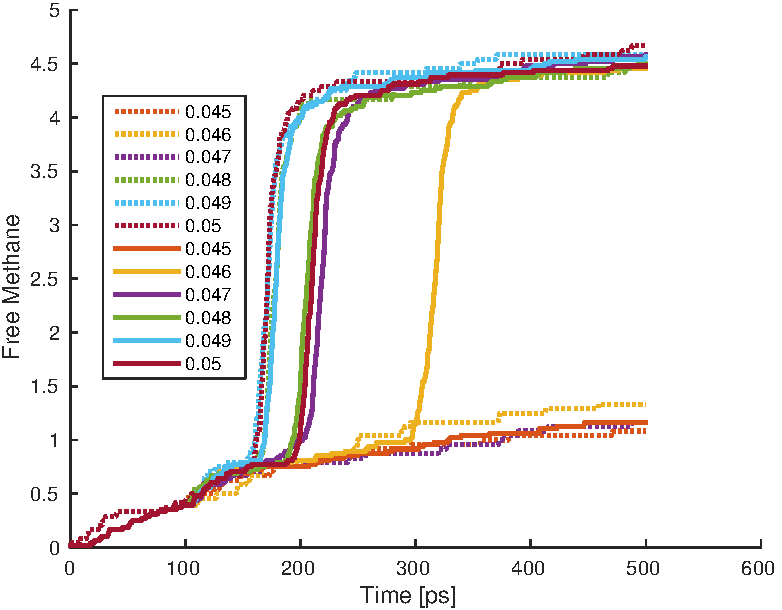
\includegraphics[width=10cm]{../figures/thesis/free_methane_nz1_nz2.pdf}
\caption{Free methane in time for systems with $L_z \approx \SI{12}{\angstrom}$ (dashed lines) $L_z\approx \SI{24}{\angstrom}$ (solid lines) for different values of the final strain (legend). Free methane is normalized by the number of unic cells in the fracture plane, so the plotted value is: $\text{Free Methane Molecules}\cdot L_{sI}^2/(L_yL_z)$.}
\label{fig:free_methane_diff_l}
\end{figure}

\subsection{Diffusion in the crack space}
Before landing on counting the number of free methanes, I explored an indirect way of measuring the amount of free methane. The idea was to assume the motion of the free methane to be diffusive. The diffusion constant could then be measured and compare to what it would have been if all methane molecules were free to move. Unfourtunately, the diffusion constant varies too much with the density of the methane gas for this to be a viable method -- both the number of methane molecules and the volume of the pore space is unknown. Furtermore, diffusion is not expected to be the same in pores as in a bulk Lennard-Jones fluid (see eg. \citet[p. 18]{Pozhar:1668293}. Therefore, this method was discarded. An additional problem is the global oscillations after crack propagation, which might furter disturb the diffusion of particles. 

But, even though measuring the number of free methanes by mean squared displacement turned out to be difficult, the diffusion constant of the free methane can still be interesting to measure. Knowing the number of free methane molecules, and assuming the rest of the methanes have exhausted their potential for contributiong to the mean squared displacement, the diffusion constant in the pore space can be measured. Figure \ref{fig:msq_methane_crack} shows the per-particle mean squared displacement of methane and water in the full-analysis simulation. The slope of the mean squared displacement is calculated to \SI{0.74}{\angstrom\squared\per\pico\second}, which corresponds to a diffusion coefficient of $D_E = \SI{1.2d-9}{\meter\squared\per\second}$. That value makes little sense, as it includes the enclathrated methane. When correcting for the fration of methane molecules that are considered free to move, in this simulation it is 2.4 \%, the diffusion coefficient of the free methane is $D_E = \SI{5.3d-8}{\meter\squared\per\second}$. This value is probably an underestimation of the diffusion coefficient for the particles that are actually diffsing, as many methanes are trapped by the wall. What can be said, however, is that this is a very high diffusion coefficient, which, given the temperature, corresponds to a low pressure. A possible simulation to compare with, is a simulation by \citet{Cao2004} of Lennard-Jones methane in carbon nanotubes. At a temperature of \SI{267}{\kelvin}, they found self-diffusion coefficients for methane of around \SI{1d-8}{\meter\squared\per\second} to \SI{10d-8}{\meter\squared\per\second} for pressures ranging from \SI{1}{\mega\pascal} to \SI{8}{\mega\pascal}. The simulations were done in carbon nanotubes with diameters from \SI{20}{\angstrom} to \SI{40}{\angstrom}. This comparison is farfetched, but it is reassuring that the results are in the right ballpark. It should be noted that the methane I observe in the crack is very dilute, possibly to the extent where Knudsen diffusion is a reasonable approximation. The methane being dilute is not obvious from the pictures of the system, since methanes that are behind each other seem to crowd the crack. If looking at the thinner system $L_z \approx \SI{12}{\angstrom}$, the diluteness becomes clear.

\begin{figure}
\centering
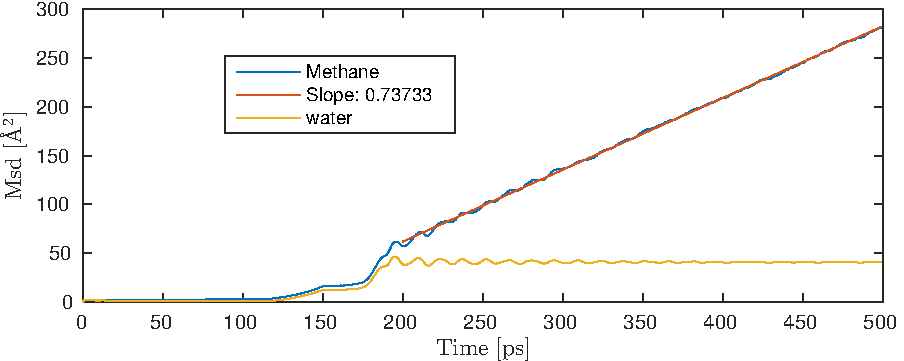
\includegraphics[width=14cm]{../figures/thesis/methane_crack_diffusion.pdf}
\caption{Per-particle mean squared displacement of methane and water in the full-analysis simulation. The slope of the methane msq is $\SI{0.74}{\angstrom\squared\per\pico\second}$.}
\label{fig:msq_methane_crack}
\end{figure}

%%%%%%%%%%%%%%%%%%%%%%%%%%%%%%%%%%%%%%%%%%%%%%%%%%%%%%
\section{Increasing the temperature}
%%%%%%%%%%%%%%%%%%%%%%%%%%%%%%%%%%%%%%%%%%%%%%%%%%%%%%
All simulations until now have been run at $T=\SI{260}{\kelvin}$. This is a relatively low temperature, and specificly, it is lower than the melting point of water for the TIP4P/ICE water model. I start by running a few simulations in the large system, $24\times 24\times 12$ sI unit cells, and report results. From then I will decide on wheter to furter investigate temperature changes.



\section{Effects of the system thickness}
The study of finite size effects has not yet gotten much attention in this work, but from visual inspection of simulations with different thicknesses $L_z$, it is clear that there are finite thickness effects. Until now, two system sizes has been studied: A thickness of one sI unit cell and a thickness of 12 sI unit cells. 

Most notably, the crack propagation in the big system is more predictable than that in the small system. Particularly, the crack tip in the small simulations can change direction for a short time, and then continue propagating in the y-direction but in another column of unit cells than it did before. Similar behavior has not been observed this in the large system.


\begin{figure}
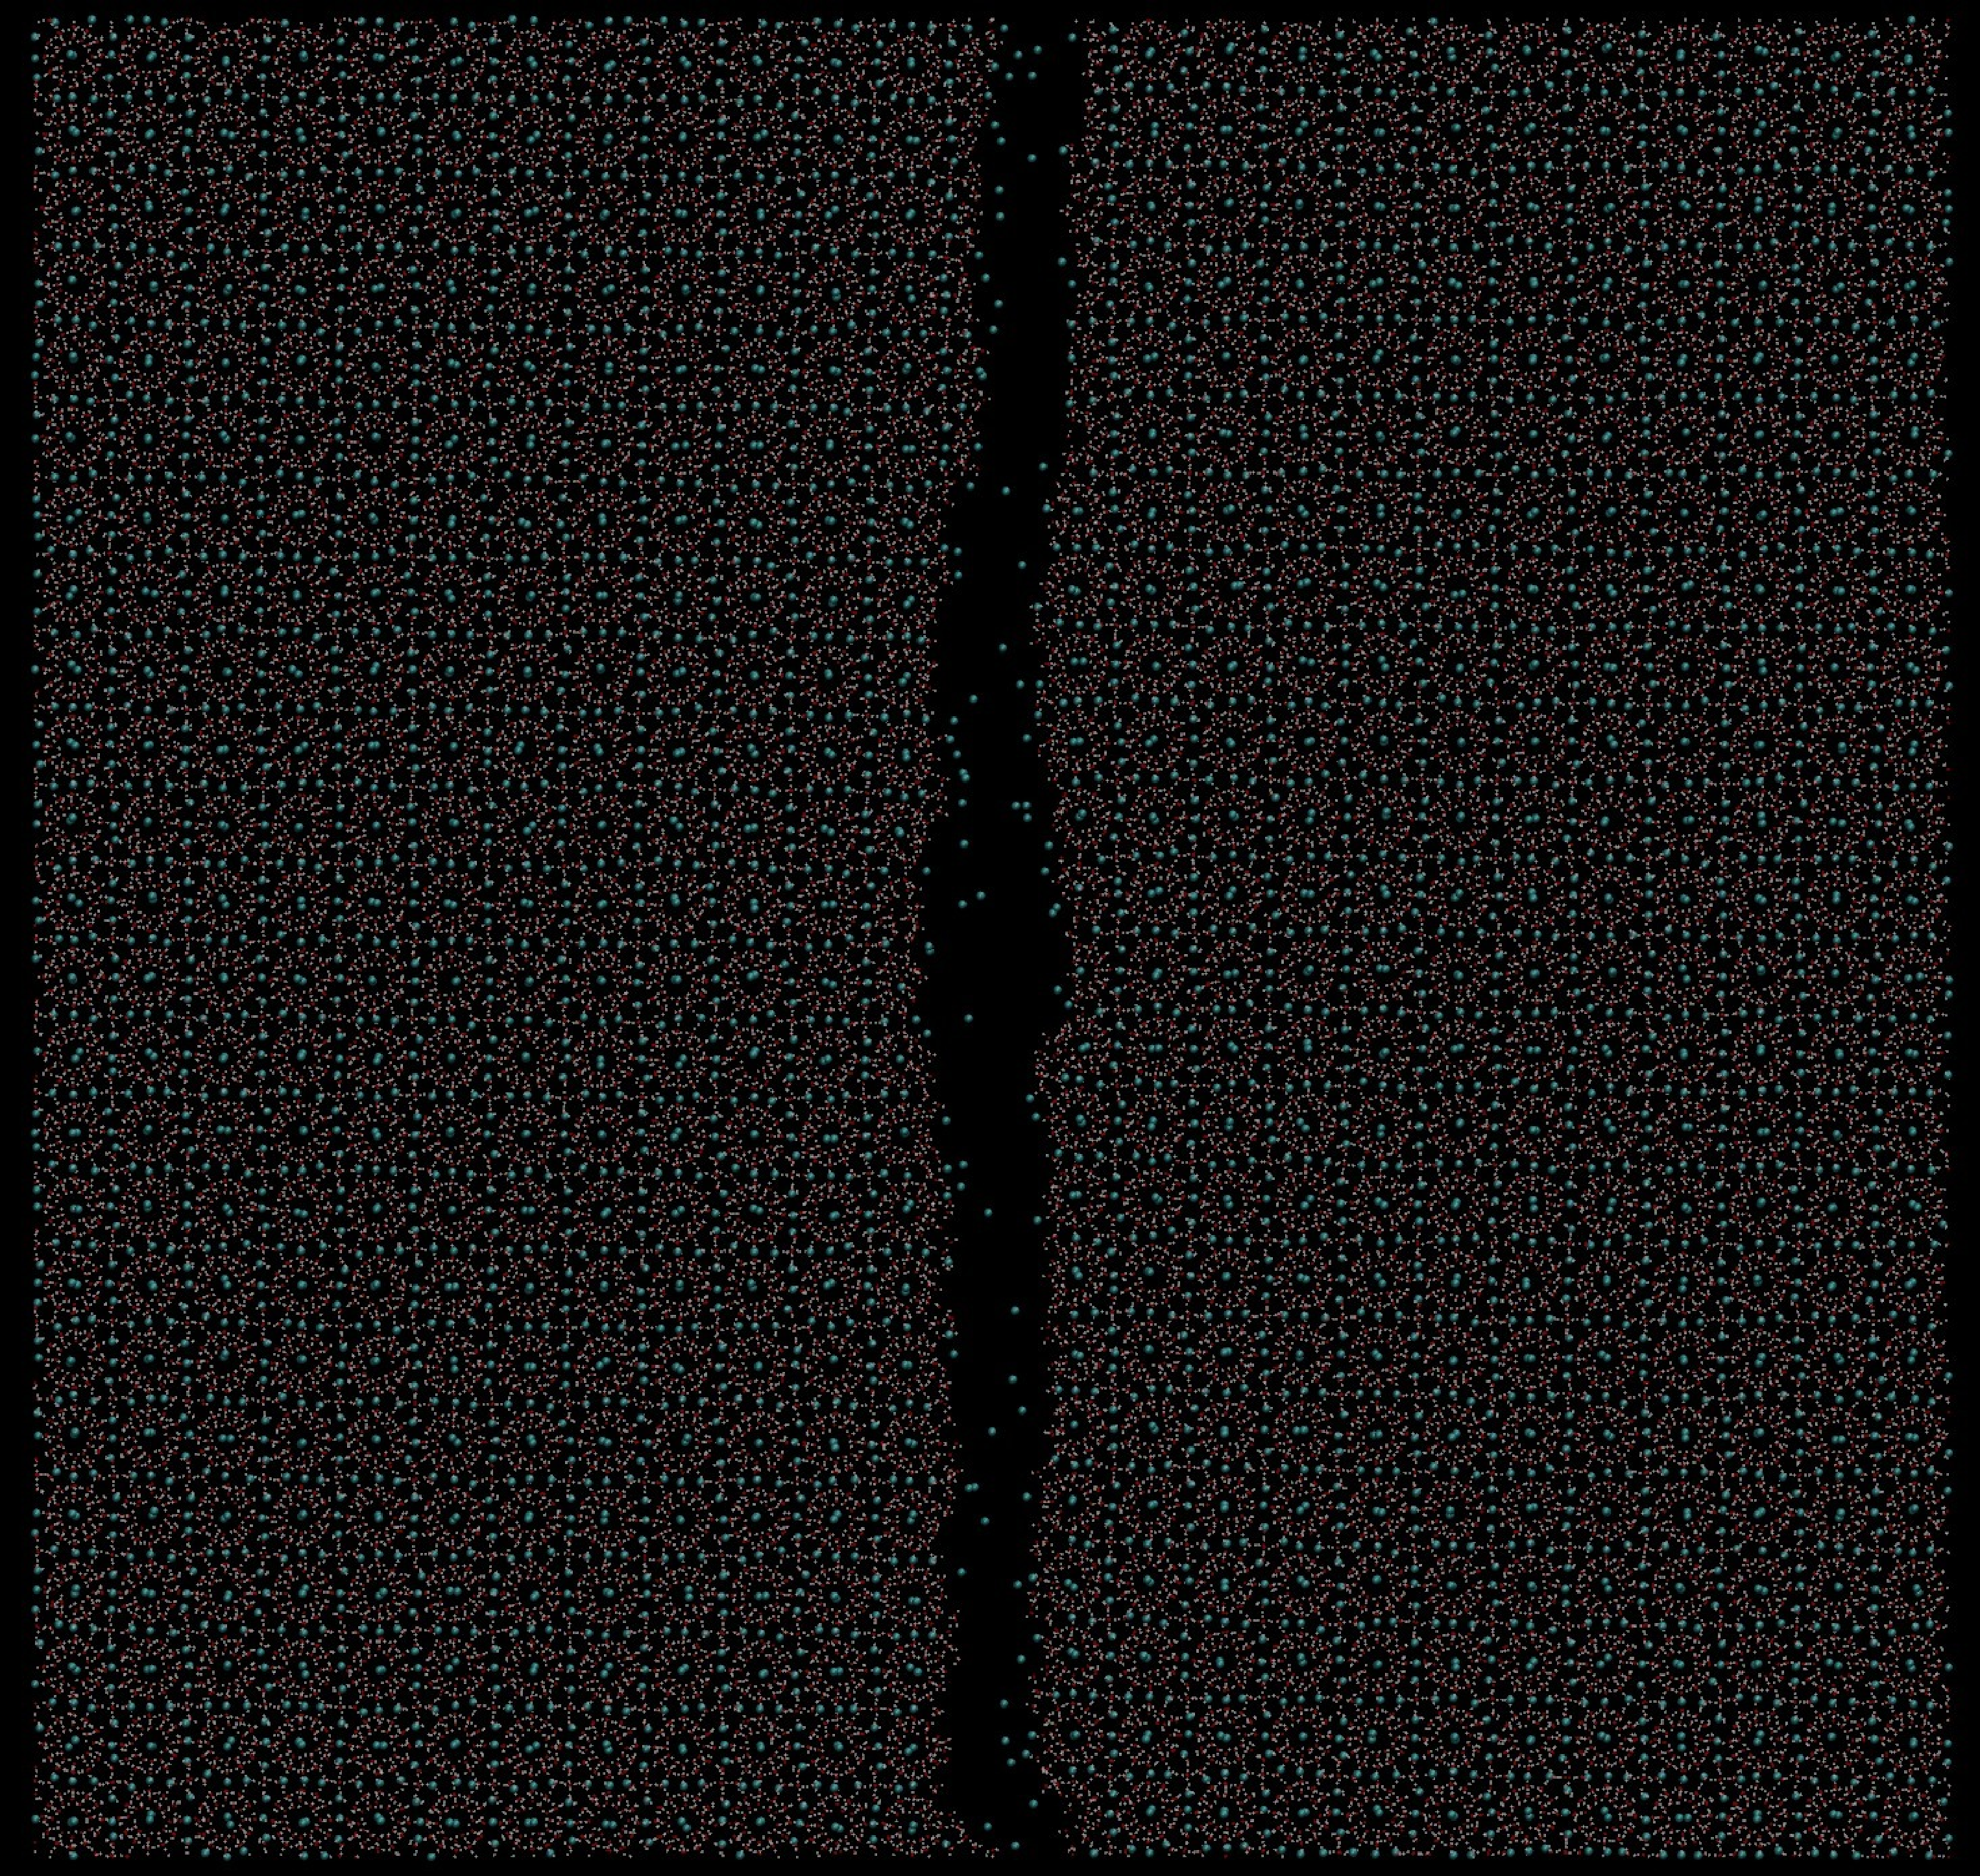
\includegraphics[width=\textwidth]{../pictures/slim_system.pdf}
\caption{Fracture of a system of $24 \times 24 \times 1$ sI unit cells. The fracture pattern is more complex than that of the thicker system: The upper crack changes from propagating between columns of unit cells to propagating in the middle of a column of unit cells, breaking big cages instead of small ones.}
\end{figure}

To systematically study this effect, I compare the crack surface area in simulations with systems of different thicknesses, but with the same strain rate. A chaotic crack should leave a larger crack surface area than a straight one.

\section{Investiagting simulations with no system-spanning crack}
All simulations up to now has had a production time of \SI{400}{\pico\second}, but as there is a waiting time before fracture starts, there might be potential of having fracture in the non-fractures systems if the simulation is sufficiently long. It is also possible that something else will happen. The crack can for example change shape and strengthen the sample. It is also possible that a much slower crack can propagate, possibly not reaching the periodic boundary if the strain does not contribute enough energy to open a surface spanning the whole yz-plane. 

In this section, I look at a simulation very similar to the one described in section \ref{sec:complete_analysis_single_simulation}. The onsly difference is that the strain level after \SI{150}{\pico\second} is 0.045, and the temperature is \SI{280}{\kelvin}. No system spanning crack is obseved during the \SI{400}{\pico\second} after straining. There is, however, a small increase in the surface area, as can be seen in figure @insertFigure. 

Since the system doesn't seem tom have equilibrated (the potential energy is still falling), I continue the simulation for another \SI{400}{\pico\second} to see what happens. Figure \ref{fig:crack_no_propagate_long_time_snapshots} shows images of the crack at selected points in time, and shos that even though the crack does not span the system after the simulations, it \emph{does} develop. It seems like the system is trying to minimize its mechanical energy by creating an optimal surface -- it looks like the crack is trying to optimize its shape. This is probably a different process than the process leading to rapid crack initiation and propagation. It can for instance be that the process can bee usefully described with a thermal activation and a stress activation. 

\begin{figure}
\begin{minipage}[b]{0.24\linewidth}
\subcaptionbox{$t=\SI{150}{\pico\second}$}{
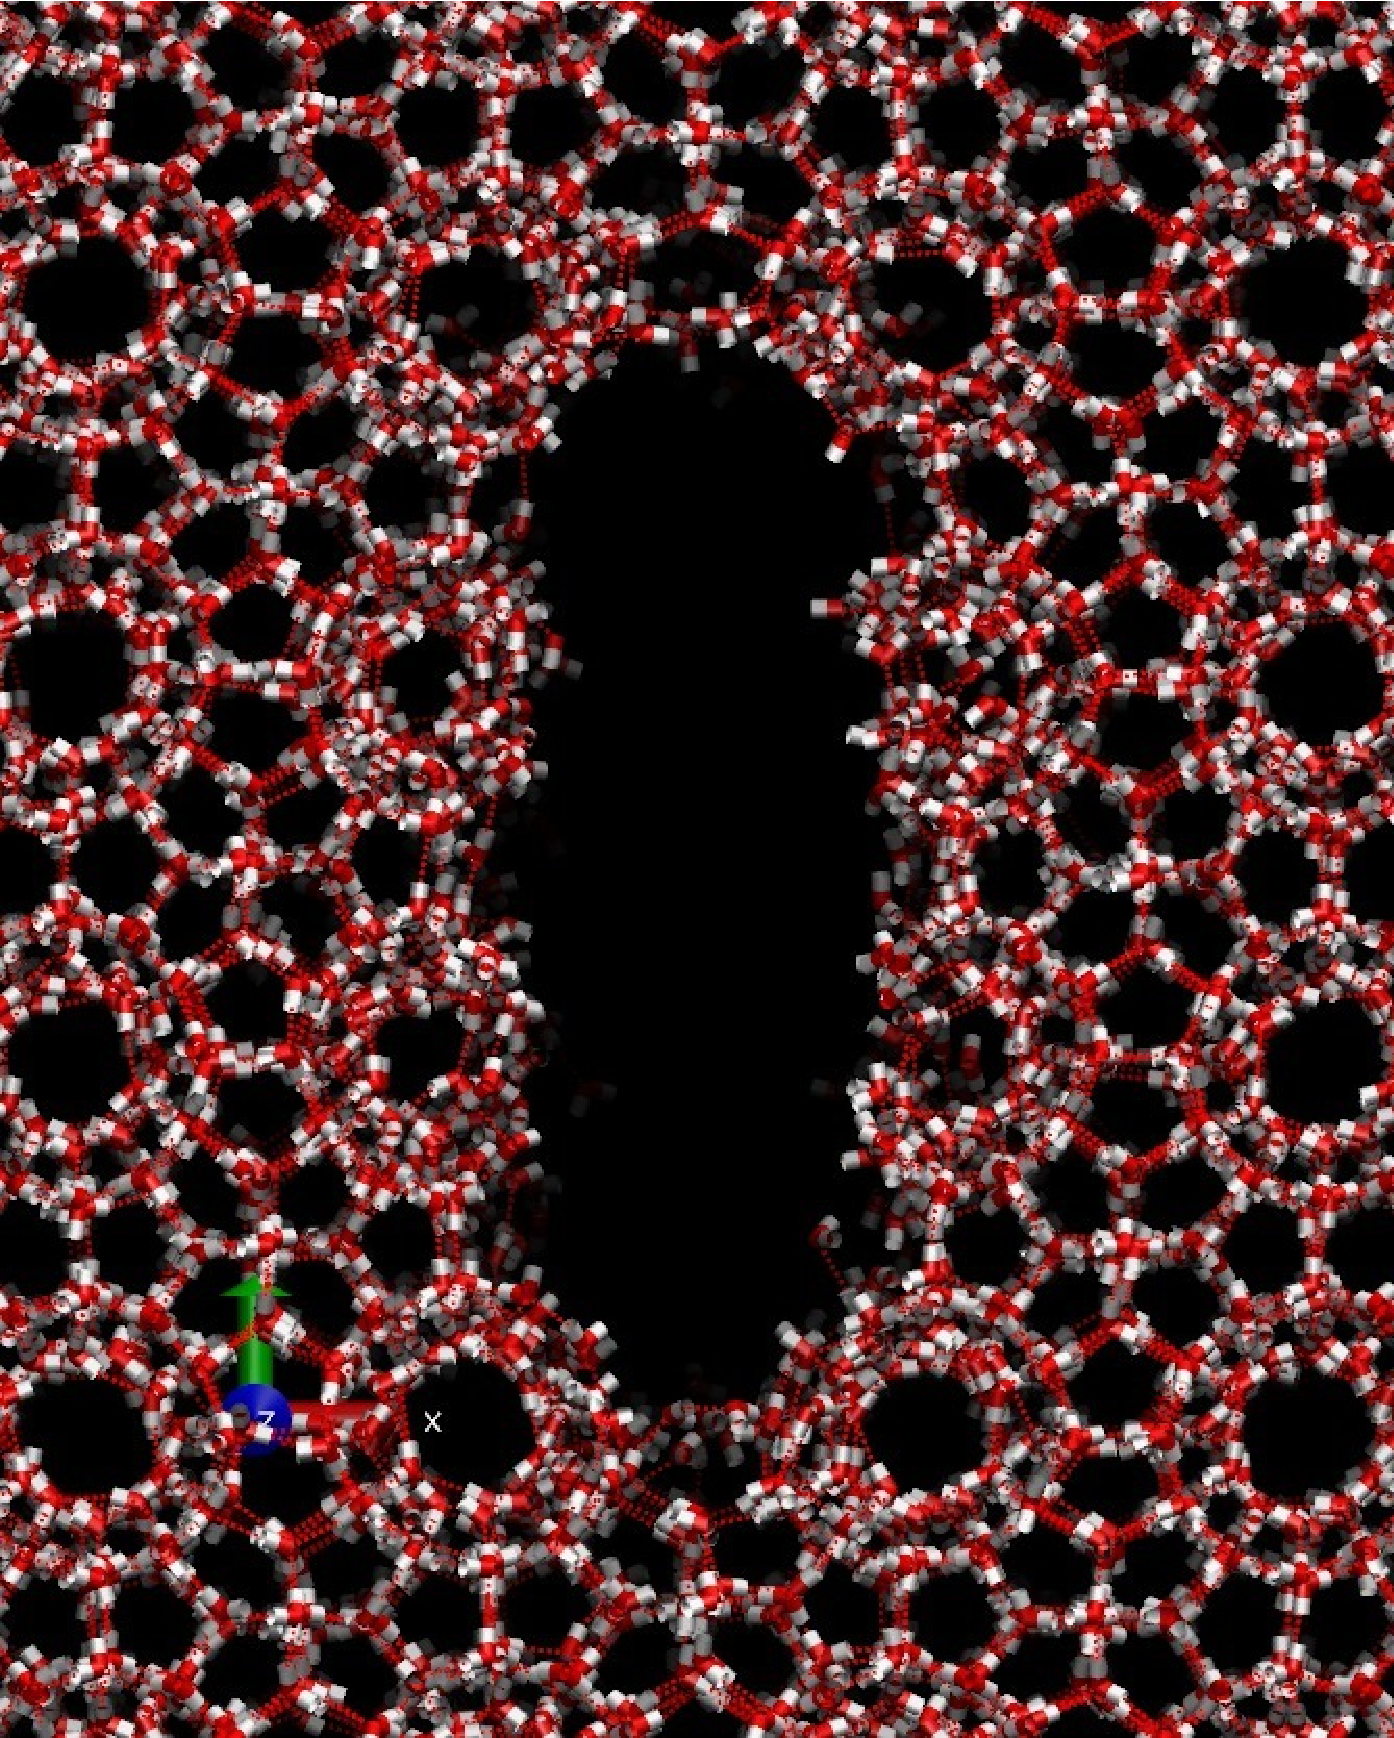
\includegraphics[width=\linewidth]{../pictures/snapshots_1045_280K/t_150000.pdf}}
\end{minipage}
\begin{minipage}[b]{0.24\linewidth}
\subcaptionbox{$t=\SI{300}{\pico\second}$}{
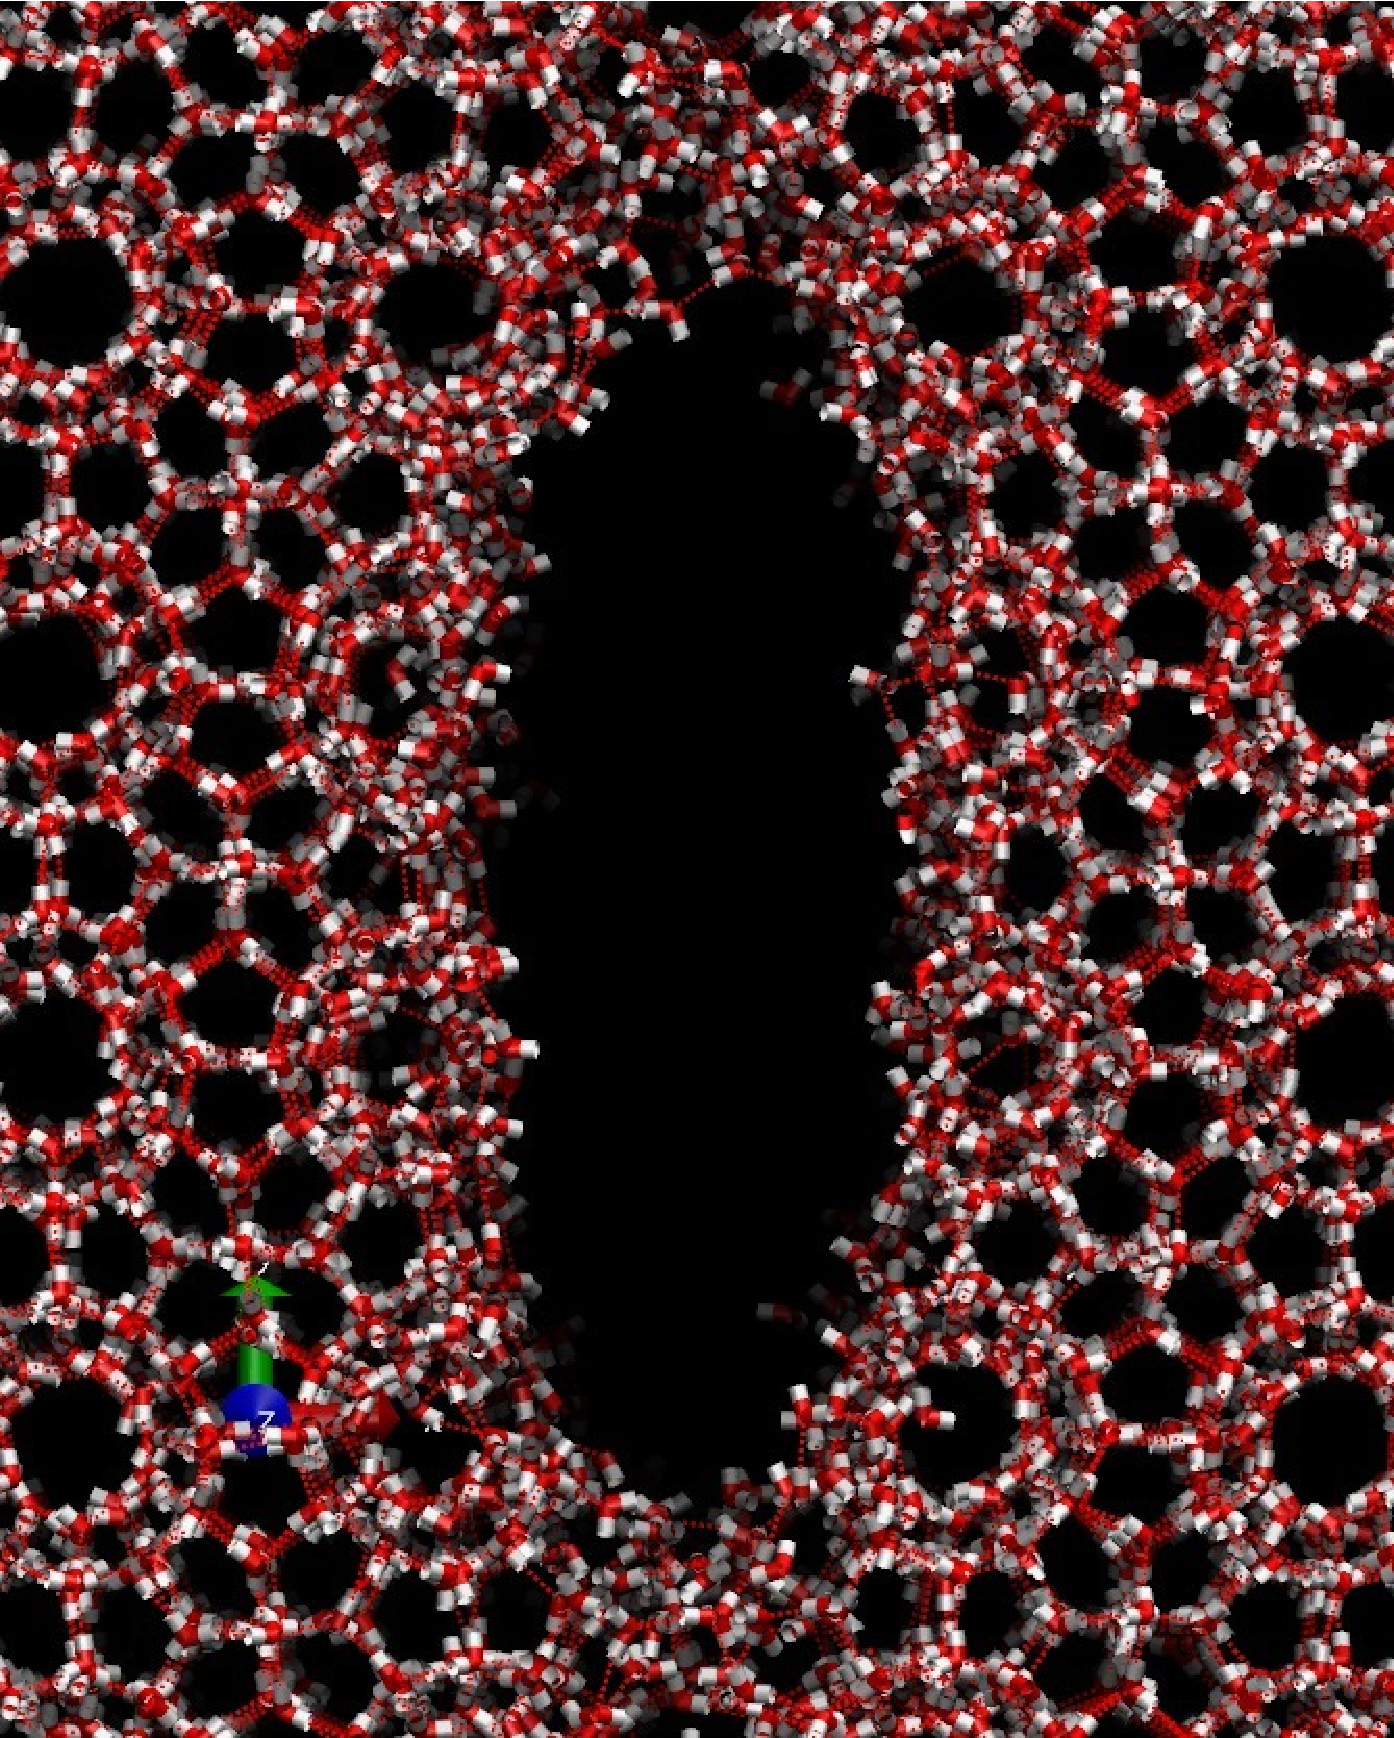
\includegraphics[width=\linewidth]{../pictures/snapshots_1045_280K/t_300000.pdf}}
\end{minipage}
\begin{minipage}[b]{0.24\linewidth}
\subcaptionbox{$t=\SI{600}{\pico\second}$}{
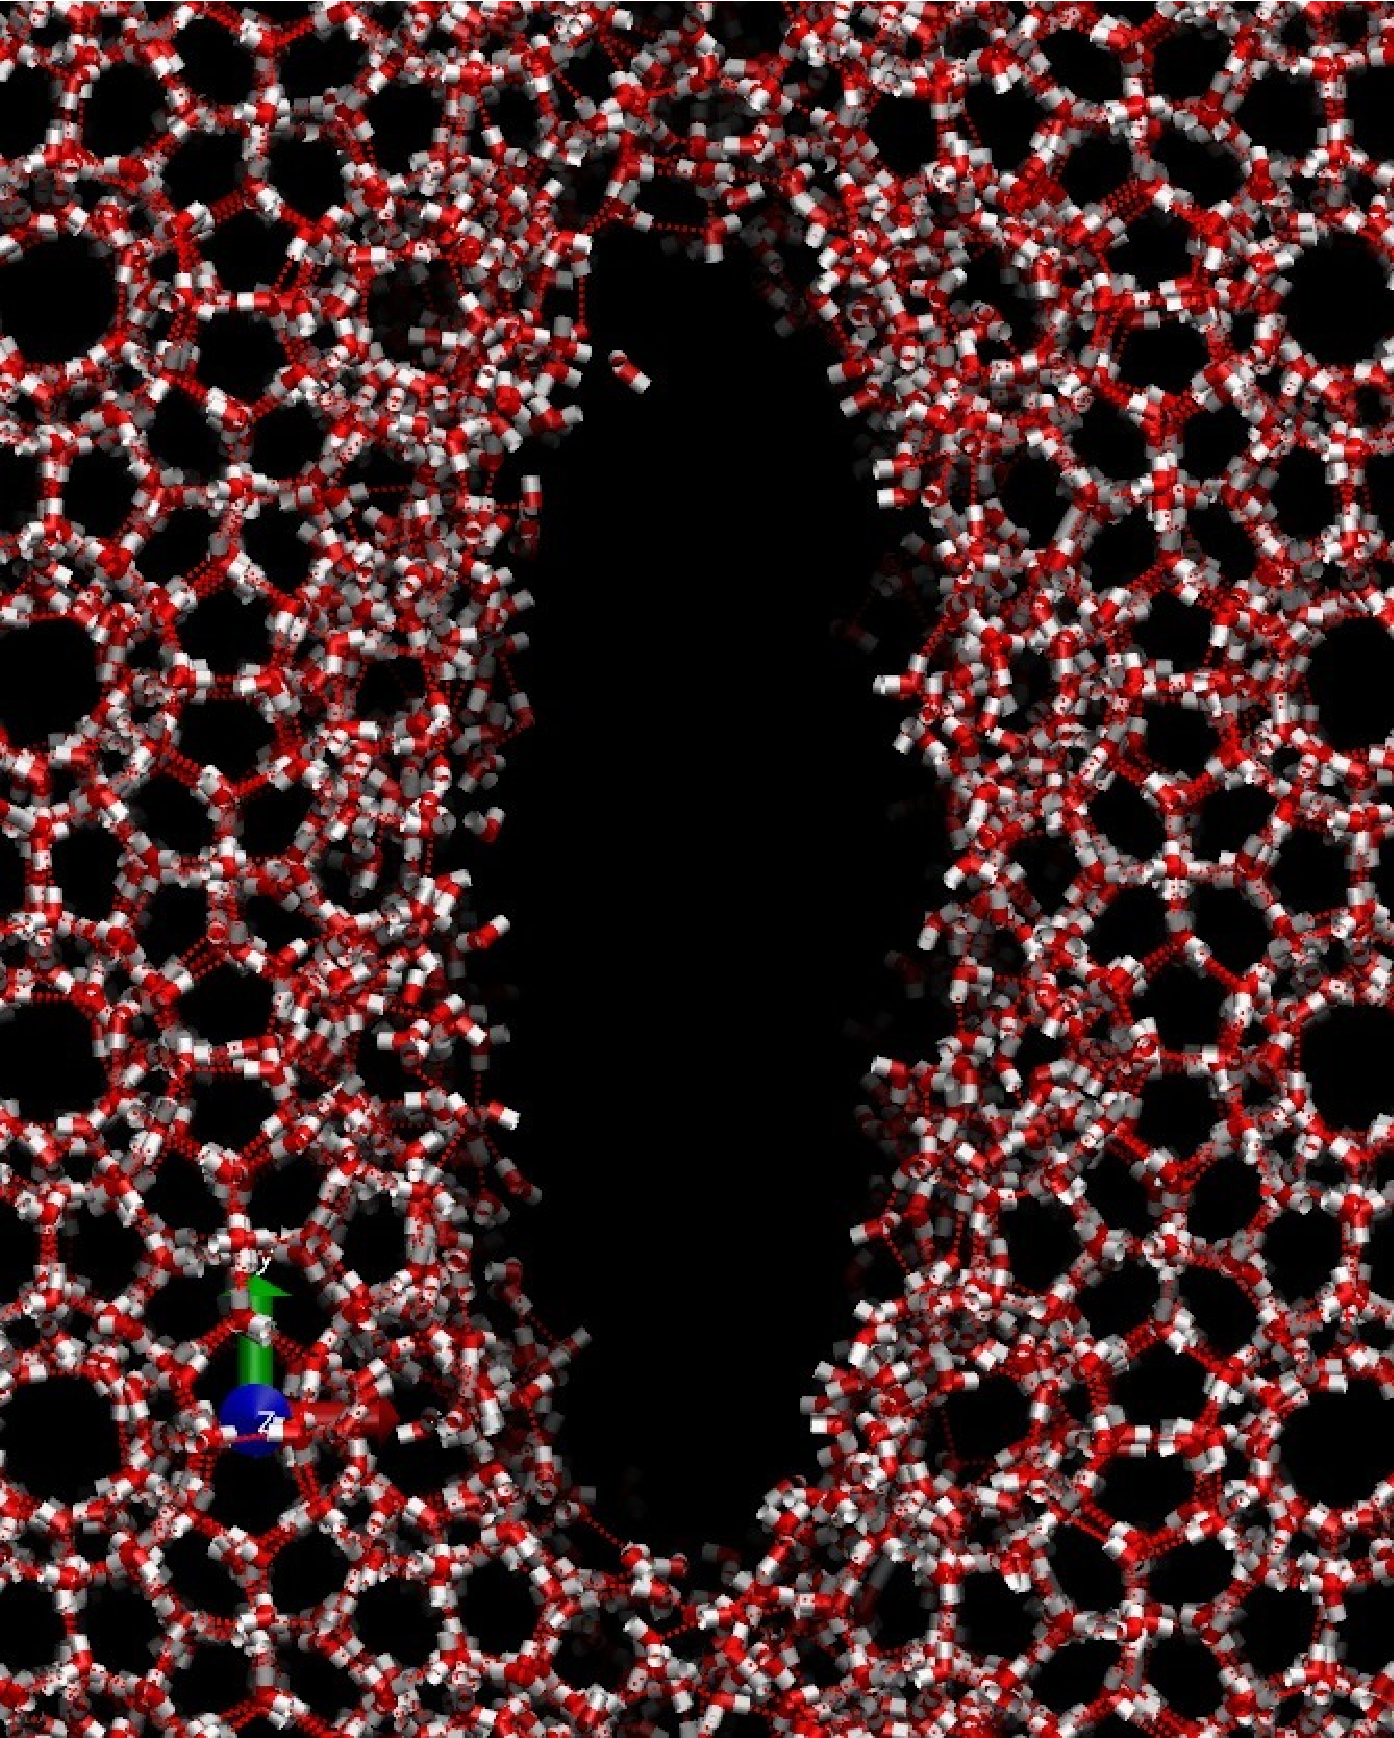
\includegraphics[width=\linewidth]{../pictures/snapshots_1045_280K/t_600000.pdf}}
\end{minipage}
\begin{minipage}[b]{0.24\linewidth}
\subcaptionbox{$t=\SI{900}{\pico\second}$}{
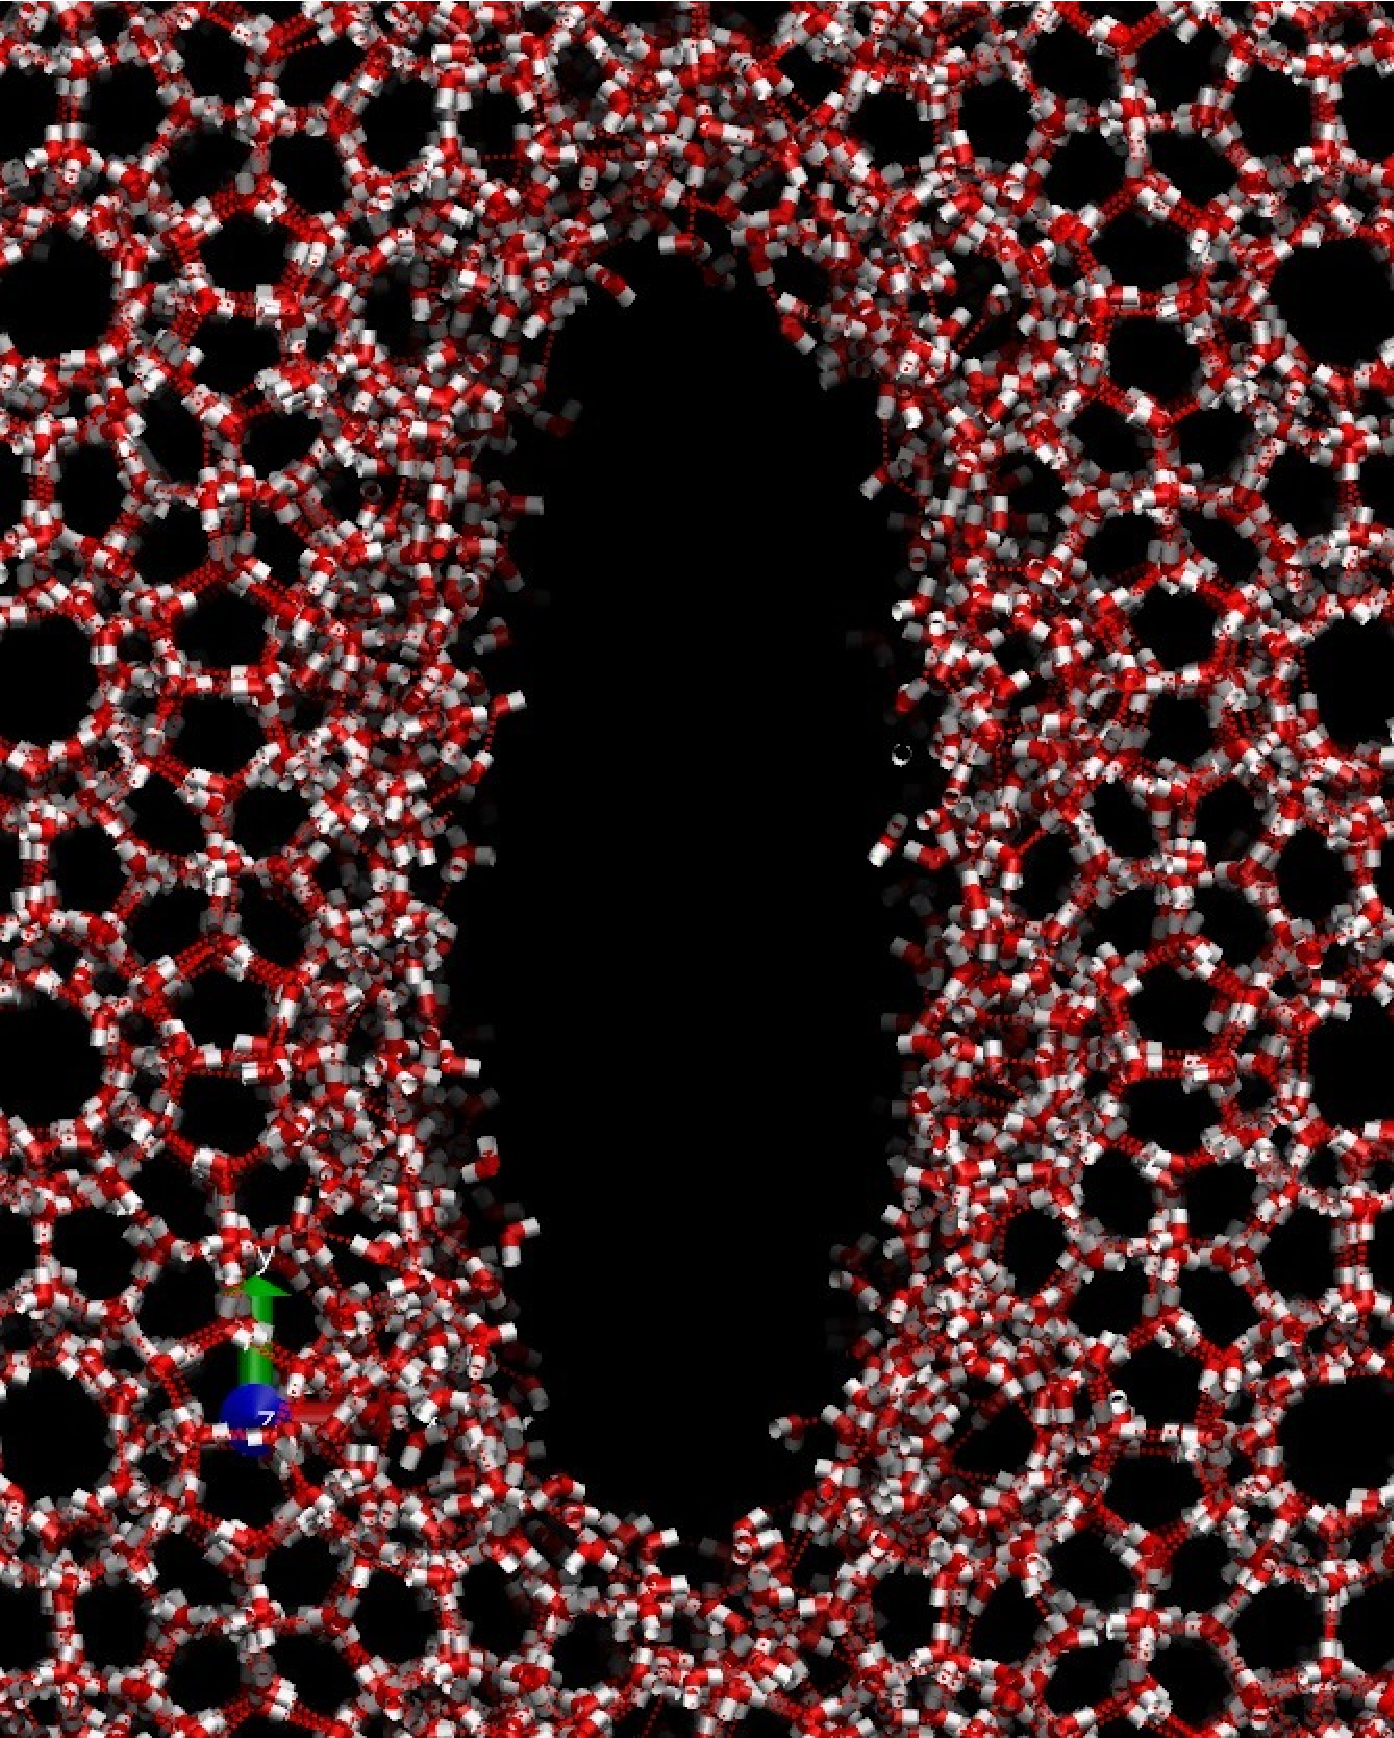
\includegraphics[width=\linewidth]{../pictures/snapshots_1045_280K/t_900000.pdf}}
\end{minipage}
\caption{Images zoomed in on the initial crack at different points in time in a long simulation. Methane molecules are hided for a better visual experience of the water. No global crack propagates, but there is still development of the small initial crack. From $t= \SI{150}{\pico\second}$ to $t=\SI{900}{\pico\second}$ the water-rich region at the wall-void interface is getting less ordered, and after $t=\SI{900}{\pico\second}$ there is a water-film between the sI hydrate and the free methane in the crack.}
\label{fig:crack_no_propagate_long_time_snapshots}
\end{figure}

\section{Aggregated results}

\subsection{Waiting time for fracture}
In the simulations with $T=\SI{260}{\kelvin}$, the waiting time was whort for the highly strained samples, and the samples subjected to too little strain didn't fracture. Between these extremes, there was no general rule that higher strains gave shorter waiting times. The simulations with $T=\SI{280}{\kelvin}$, on the other hand, showed more systematic behavior, and generally shorter waiting times. It is possible that the variation in waiting time is smaller when temperature increases, and especially when exceeding the melting temperature of pure water in the given model.

\begin{figure}
\centering
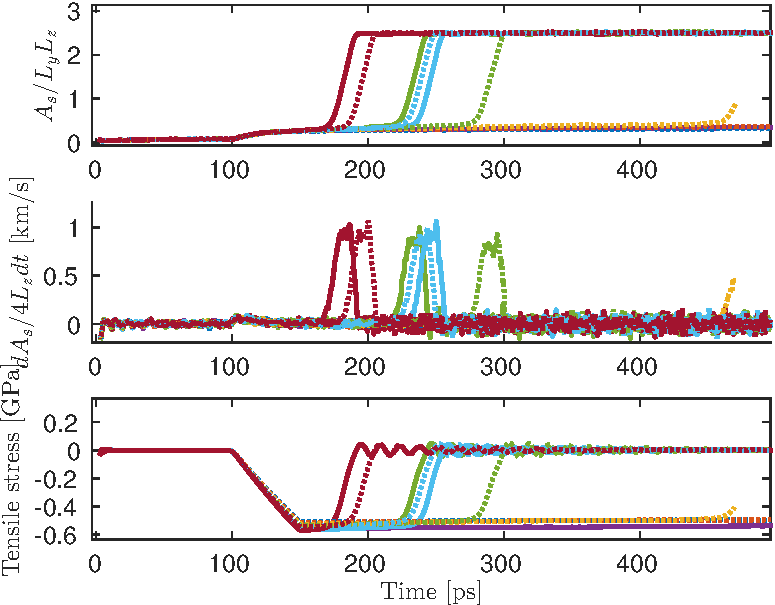
\includegraphics[width=12cm]{../figures/thesis/area_speed_stress_all.pdf}
\caption{Crack area (top panel), crack speed (middle panel) and tensile stress (lower panel). Simulation temperatures are \SI{260}{\kelvin} (solid lines) and \SI{280}{\kelvin} (dashed lines). Strains: 0.044 (blue) 0.045 (orange), 0.046 (yellow), 0.0465 (violet), 0.047 (green), 0.0475 (cyan), 0.048 (purple). The colors are the same as in the legend of figure \ref{fig:fracture_theory_compare}. }
\label{fig:area_speed_stress_all}
\end{figure}

\begin{figure}
\centering
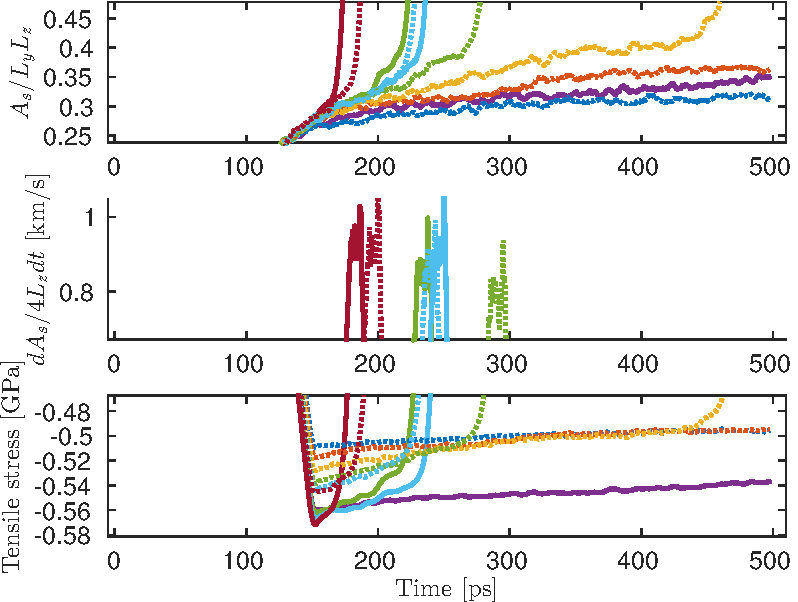
\includegraphics[width=12cm]{../figures/thesis/area_speed_stress_all_zoomed.pdf}
\caption{Crack area (top panel), crack speed (middle panel) and tensile stress (lower panel). The panels are the same as the ones in \ref{fig:area_speed_stress_all}, but they are significantly zoomed.}
\end{figure}

\subsection{Crack tip speed}
There is a significant relationship between the crack tip speed and the strain before fracture. 

\subsection{Free methane}
Methane is freed almost instantly during crack propagation, which is opposed to the possibility of a very sharp crack where methane would have to diffuse out of their cages after crack propagation. It is also worth noting that the proportion of methane that is freed during rapid surface area growth is of the same order as the proportion of surface area that is grown during rapid area growth. That means methane is quickly released -- it does not stay in the mydrate lattice and then diffuse out.


\subsection{Surface energy}
Measured surface energy for different configurations:

\begin{table}
\centering
\begin{tabular}{c|c}
Parameters & Surface energy \\
\hline
\SI{280}{\kelvin}, $L_Z = \SI{145}{\angstrom}$ & \SI{0.21 \pm 0.01}{\joule\per\meter\squared}
\end{tabular}
\end{table}

\section{Comparison with continuum LEFM}
Figure \ref{fig:fracture_theory_compare} shows the global tensile stress in the \SI{280}{\kelvin} simulations plotted against the crack length. The results agree well with the Griffith thory for brittle solids. It might be that this plot can aid the understanding of two separate mechanisms for fracture. some process slowly increases the crack width and reduces the tensile stress, until -- at some point -- the crack width-tensile stress configuration is such that it allows for rapid crack growth. This should be determined by whether the simulation follows a less steep slope than some critical line, which is probably close to the finite width Griffith line.
\begin{figure}
\centering
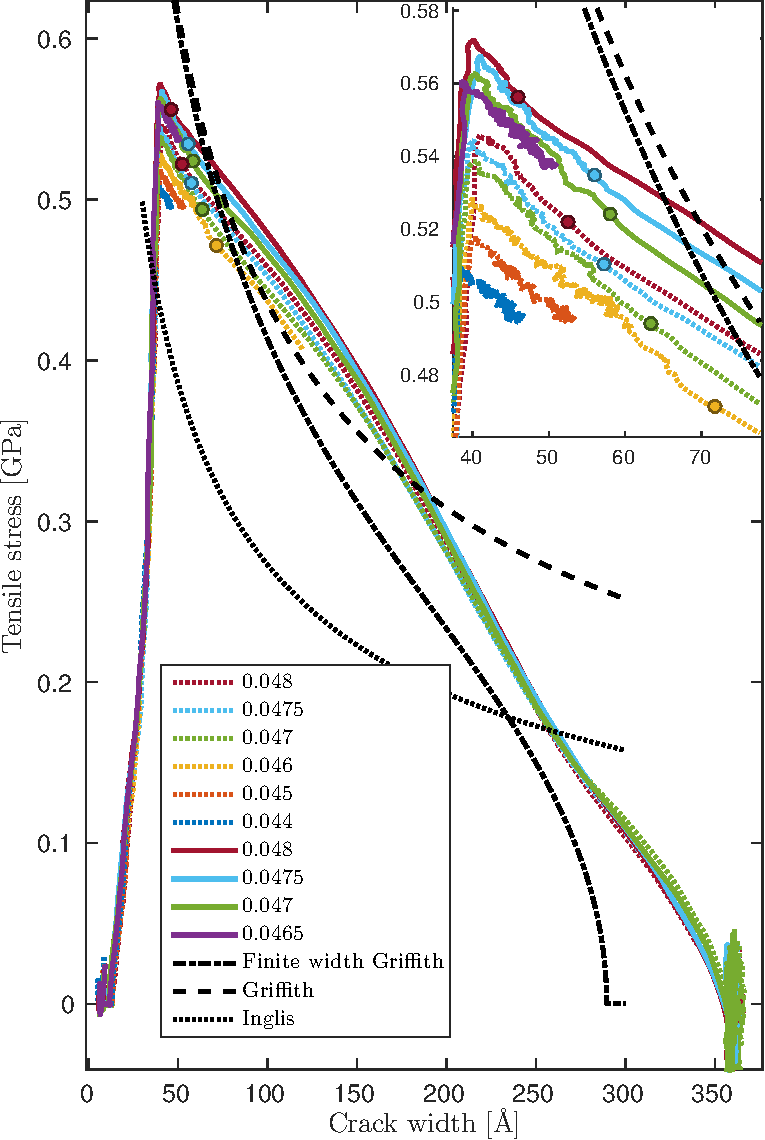
\includegraphics[width=12cm]{../figures/thesis/stress_area_lefm.pdf}
\caption{Relationship between tensile stress and crack width during dynamic runs. Markers indicate where critial fracture is estimated to have started (judgement call from looking at the fracture speed). It is the position of the markers that determine whether this is a good agreement with Griffith or Inglis theory. The crack width is estimated as $A_s/2L_z$, and it is clear that it is over-estimated at the end of the simulation (at full crack opening). It is not clear whether the crack length is over-estimated at the early stages of crack propagation. When straining is finished, which is at the point where the stress reaches its maximum, the crack area is quite exactly estimated to the length of the crack that was carved out, namely \SI{40}{\angstrom}. The theory curves (Inglis and Griffith) are calculated using $E=\SI{7.1}{\giga\pascal}$ and $\gamma_s = \SI{0.21}{\joule\per\meter\squared}$ The finite width curve is made using equation \ref{eq:griffith_finite_sheet}. The legend indicate the maximum strain level in each simulation, and the diffenrent theoretical curves.}
\label{fig:fracture_theory_compare}
\end{figure}